\documentclass{article}
\usepackage{amsmath, amssymb, tikz, geometry, graphicx, natbib, mwe, color, xcolor, listings, tabularx, pdfpages, blindtext, mathtools, stackengine, pgfplots,bigints, relsize, upgreek, esint, array, multirow, schemata, wrapfig, cancel, comment}
\usepackage{hyperref}
\usepackage{slashed, enumitem}
\usepackage{titlesec}
\usepackage[export]{adjustbox}
\usetikzlibrary{positioning}

\begin{comment}
code to write section, subsection and subsubsection title in a specific color
\titleformat{\section}
{\color{synthwave_text}\normalfont\Large\bfseries}
{\color{synthwave_text}\thesection}{1em}{} 

\titleformat{\subsection}
{\color{synthwave_text}\normalfont\large\bfseries}
{\color{synthwave_text}\thesubsection}{1em}{} 

\titleformat{\subsubsection}
{\color{synthwave_text}\normalfont\normalfont\bfseries}
{\color{synthwave_text}\thesubsubsection}{1em}{}
\end{comment}

%code to have equation like subsection (1.1,1.2,...)
\numberwithin{equation}{subsection}

\let\oldsection\section% Store \section
\renewcommand{\section}{% Update \section
  \renewcommand{\theequation}{\thesection.\arabic{equation}}% Update equation number
  \oldsection}% Regular \section
\let\oldsubsection\subsection% Store \subsection
\renewcommand{\subsection}{% Update \subsection
  \renewcommand{\theequation}{\thesubsection.\arabic{equation}}% Update equation number
  \oldsubsection}% Regular \subsection


\pgfplotsset{compat=1.9}

\colorlet{myWhite}{white!35!gray}
\definecolor{shadeofgray}{HTML}{181818}
\definecolor{shadeofviolet}{HTML}{0f022c}
\definecolor{synthwave_beckground}{HTML}{252334}
\definecolor{synthwave_text}{HTML}{e148aa}


\hypersetup{
    colorlinks=true,
    linkcolor=violet,
    filecolor=magenta,      
    urlcolor=cyan,
    pdftitle={Controlli Automatici T},
    pdfpagemode=FullScreen,
}


\geometry{ 
 a4paper,
 left=10mm,
 right=10mm,
 top=10mm
 }
 
\lstdefinestyle{mystyle}{ 
bracketsstyle=\color{red}
}

\title{Controlli Automatici T}
\author{Giuseppe Bumma}


% color option
%\pagecolor{synthwave_beckground} %{shadeofgray}
%\color{myWhite}



\begin{document}

%Commands
\newcommand{\R}{\mathbb{R}}
\newcommand{\Varepsilon}{\mathcal{E}}
\newcommand{\rad}{\text{rad}}
\newcommand{\bb}[1]{\mathbb{#1}}
\newcommand{\cc}[1]{\mathcal{#1}}
\newcommand{ \lognormal }{\text{Lognormal} }
\newcommand{\T}[1]{\text{#1}}
\newcommand*\circled[1]{\tikz[baseline=(char.base)]{%
            \node[shape=circle,draw,inner sep=2pt] (char) {#1};}}
%for using circled number in enumerate use:
%\begin{enumerate}[label=\protect\circled{\arabic*}]


\tableofcontents

\maketitle

\section{Introduzione}
L'idea dei \textbf{controlli automatici} è sostituire l'intelligenza umana con un sistema automatico (come l'intelligenza artificiale) basata su leggi matematiche e/o algoritmi.



\subsection{Notazione ed elementi costitutivi}
\begin{center}
    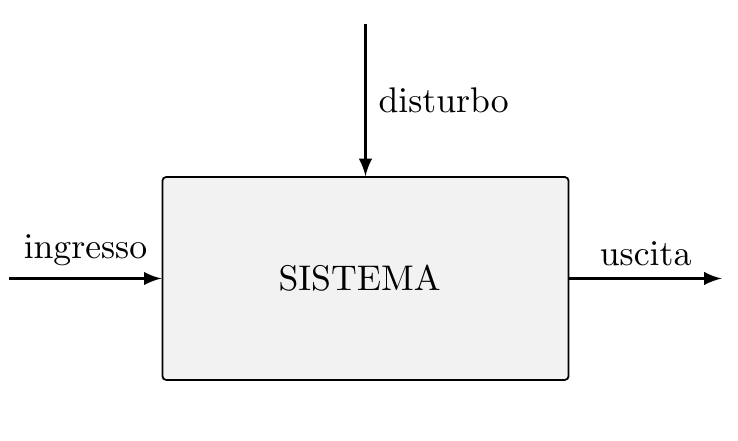
\includegraphics[scale=0.3]{Images/Schema_sistema.png}
\end{center}
Il \textbf{sistema} è un oggetto per il quale si vuole ottenere un comportamento desiderato.
\\
Esempi di sistema sono: impianto (industriale), macchinario (braccio robotico, macchina a controllo numerico, etc\dots), veicolo (auto, velivolo, drone, etc\dots), fenomeno fisico (condizioni atmosferiche), sistema biologico, sistema sociale.
\\
L'obiettivo è che l'andamento nel tempo di alcune variabili segua un segnale di riferimento.
\vspace*{0.2cm}\\
Altri elementi sono:
\begin{itemize}
    \item Controllore: unità che determina l'andamento della variabile di controllo (ingresso);
    \item Sistema di controllo: sistema (processo) + controllore;
    \item Sistemi di controllo naturali: meccanismi presenti in natura, come  quelli presenti nel corpo umano (temperatura corporea costante, ritmo cardiaco, etc\dots);
    \item Sistemi di controllo manuali: è presente l'azione dell'uomo;
    \item Sistemi di controllo automatico: uomo sostituito da un dispositivo.
\end{itemize}




\subsection{Controllo in anello aperto e anello chiuso}
Controllo in anello aperto (“feedforward”): il controllore utilizza solo il segnale di riferimento
\begin{center}
    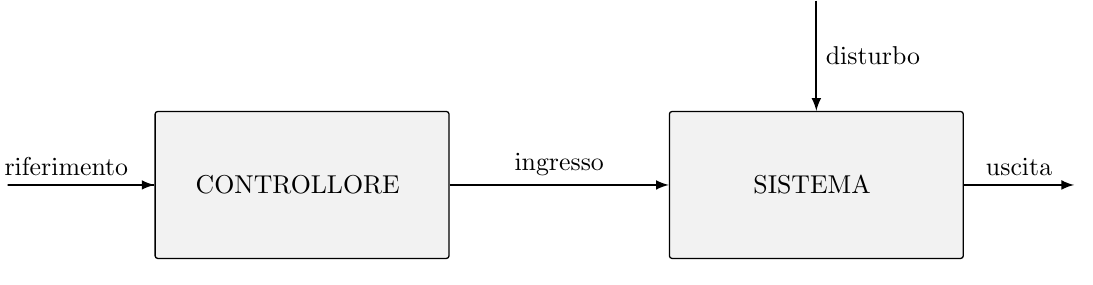
\includegraphics[scale=0.32]{Images/Anello_aperto.png}
\end{center}
Controllo in anello chiuso (“feedback” o retroazione): il controllore utilizza il segnale di riferimento e la variabile controllata ad ogni istante di tempo
\begin{center}
    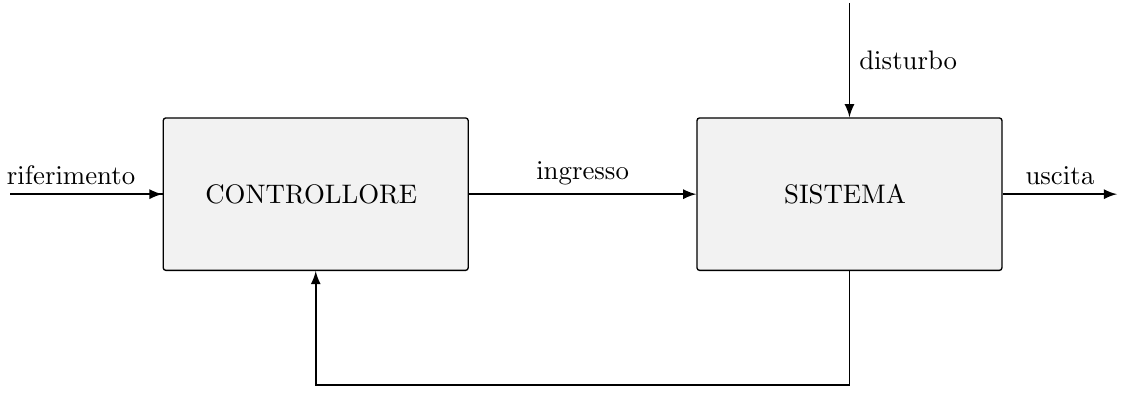
\includegraphics[scale=0.3]{Images/Anello_chiuso.png}
\end{center}
Il controllo in retroazione è un paradigma centrale nei controlli automatici.


\subsection{Progetto di un sistema di controllo}
I passi passi per progettare un sistema di controllo sono:
\begin{itemize}
    \item definizione delle specifiche: assegnazione comportamento  desiderato, qualità del controllo, costo,...
    \item modellazione del sistema (controllo e test): complessità del modello (compromesso), definizione ingressi/uscite, codifica del modello, validazione in simulazione
    \item analisi del sistema: studio proprietà “strutturali”, fattibilità specifiche
    \item sintesi legge di controllo: è basata su modello, analisi sistema controllato, stima carico computazionale
    \item simulazione sistema controllato: test su modello di controllo, test realistici (modello complesso, ritardi, quantizzazione, disturbi, ...)
    \item scelta elementi tecnologici: sensori/attuatori, elettronica di acquisizione/attuazione, dispositivo di elaborazione
    \item sperimentazione: hardware in the loop, prototipazione rapida, realizzazione prototipo definitivo
\end{itemize}





\subsection{Esempio di sistema di controllo: circuito elettrico} \label{Circuito elettrico}
\begin{center}
    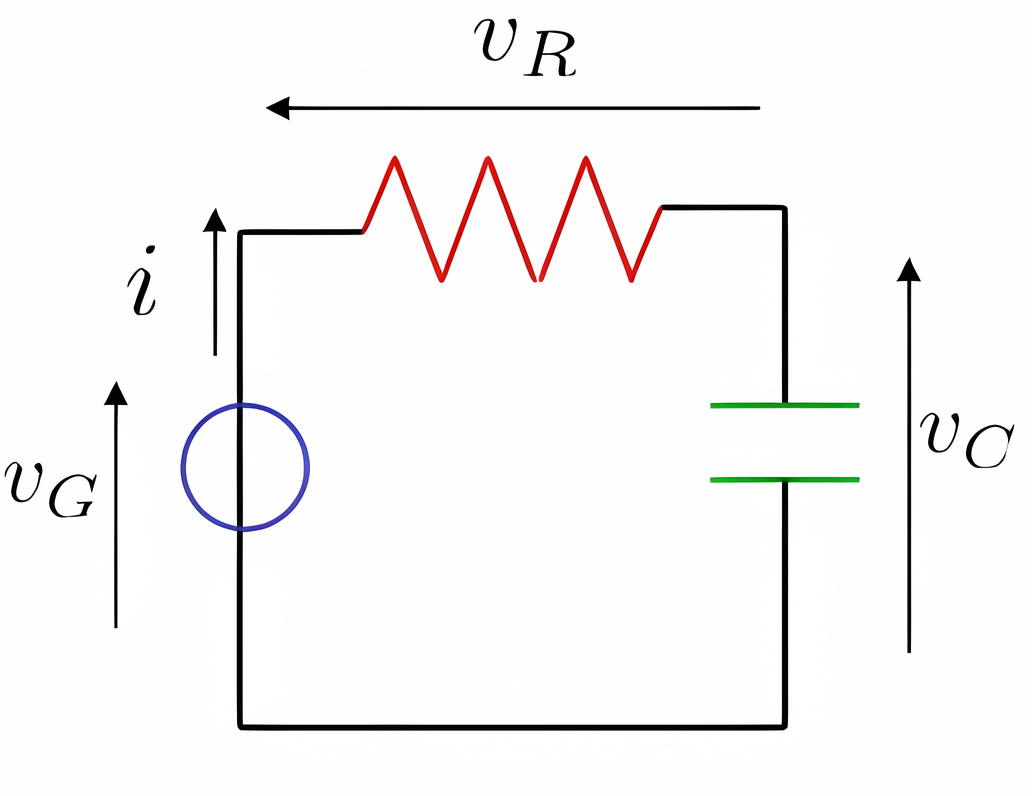
\includegraphics[scale=0.2]{Images/Es_cirucito_elettrico.png}
\end{center}
La legge che usiamo per definire il circuito (il nostro sistema) è la \textit{legge delle tensioni}
\begin{equation}
    v_R (t) = v_G (t) - v_C(t)
\end{equation} 
le leggi del condensatore e del resistore sono 
\begin{align*}
    C \cdot  \dot v_C (t) &= i(t) & v_R (t) = R\cdot i(t)
\end{align*}
Scrivendo la formula in termini di $v_C (t)$ (“stato interno”) e $v_G (t)$ (“ingresso di controllo”)
\begin{equation}
    \dot v_C (t) = \frac{1}{RC} \left(v_G (t) - v_C (t) \right)
\end{equation}




\section{Sistemi in forma di stato}
\subsection{Sistemi continui}
I \textit{sistemi continuti} sono sistemi in cui il tempo è una variabile reale: $t \in \mathbb{R}$
\begin{align*}
    \dot x(t) &= f \left( x(t), u(t), t \right) & &\text{equazione di stato}\\
    \dot y(t) &= h\left(x(t), u(t), t\right) & &\text{equazione  (trasformazione) di uscita }
\end{align*}
Definiamo inoltre $t_0$ come tempo iniziale e $x(t_0)=x_0$ come stato iniziale. \\
\textbf{N.B.} $\dot x(t) := \dfrac{d}{dt}x(t)$.
\vspace*{0.1cm}\\
Notazione:
\begin{itemize}
    \item $x(t) \in \mathbb{R}^n$ stato del sistema all'istante $t$
    \item $u(t) \in \mathbb{R}^m$ ingresso del sistema all'istante $t$
    \item $y(t) \in \mathbb{R}^p$ uscita del sistema all'istante $t$
\end{itemize}
\begin{equation}
    x(t)=
    \begin{bmatrix}
        x_1(t)\\
        ...\\
        ...\\
        ...\\
        x_n(t)
    \end{bmatrix}
    \ \ \ \ \ 
    u(t) =
    \begin{bmatrix}
        u_1(t)\\
        ...\\
        ...\\
        ...\\
        u_m(t)
    \end{bmatrix}
    \ \ \ \ \ 
    y(t) = 
    \begin{bmatrix}
        y_1(t)\\
        ...\\
        ...\\
        ...\\
        y_p(t)
    \end{bmatrix}
\end{equation}
Da notare che $x(t)$ è un vettore mentre $x_1,...,x_n$ sono scalari.\\
$x(t)$ è una variabile interna che descrive il comportamento del sistema.


\subsubsection{Equazione di stato}
L'\textit{equazione di stato} è un'equazione ordinaria (ODE) vettoriale del primo ordine (cioè l'ordine massimo delle derivate è 1)
\begin{align*}
    \dot x_1(t) &= f_1 \left(x(t), u(t), t\right)\\
    &\dots\\
    \dot x_n (t) &= f_n \left(x(t), u(t), t\right)
\end{align*}
$\mathbb{R}^n$ è detto \underline{spazio di stato}, con $n$ ordine del sistema. La funzione di stato è $f: \mathbb{R}^n \times \mathbb{R}^m \times \mathbb{R} \rightarrow \mathbb{R}^n$.
\begin{equation}
    \begin{bmatrix}
        \dot x_1(t)\\
        ...\\
        ...\\
        ...\\
        \dot x_n(t)
    \end{bmatrix} 
    =
    \begin{bmatrix}
        f_1\left(x(t),u(t),t\right)\\
        ...\\
        ...\\
        ...\\
        f_n\left(x(t),u(t),t\right)
    \end{bmatrix}
    := f\left(x(t),u(t),t\right)
\end{equation}
Avere solo derivate prime non è limitato, perché ad esempio posso inserire una prima variabile come derivata prima e una seconda variabile come derivata prima della prima variabile.

\subsubsection{Equazione di uscita}
L'equazione di uscita è un'equazione algebrica
\begin{align*}
    y_1(t) &= h_1 \left(x(t), u(t), t\right)\\
    &\dots\\
    y_p (t) &= h_p \left(x(t), u(t), t\right)
\end{align*}
$h : \mathbb{R}^n \times \mathbb{R}^m , \mathbb{R} \rightarrow R^p$ funzione di uscita
\begin{equation}
    \begin{bmatrix}
        y_1(t)\\
        ...\\
        ...\\
        ...\\
        y_p(t)
    \end{bmatrix} 
    =
    \begin{bmatrix}
        h_1\left(x(t),u(t),t\right)\\
        ...\\
        ...\\
        ...\\
        h_p\left(x(t),u(t),t\right)
    \end{bmatrix}
    := h\left(x(t),u(t),t\right)
\end{equation}
\vspace*{0.2cm}
Se la soluzione $x(t)$ a partire da un istante iniziale $t_0$ è univocamente determinata da $x(t_0)$ e $u(\tau)$ con $\tau \geq t_0$, allora il sistema è detto \textbf{causale}, cioè lo stato dipende solo da ciò che accede in passato.\\
Sotto opportune ipotesi di regolarità della funzione $f$ si dimostra esistenza e unicità della soluzione dell'equazione (differenziale) di stato (Teorema di Cauchy-Lipschitz).



\subsection{Sistemi discreti}
Nei \textit{sistemi discreti} il tempo $t$ è una variabile intera, $t \in \mathbb{Z}$.
\begin{align*}
    x(t+1) &= f \left(x(t), u(t), t\right) & &\text{equazione di stato}\\
    y(t) &= h\left(x(t), u(t), t\right) & &\text{equazione (trasformazione) di uscita}
\end{align*}
L'equazione di stato è un'equazione alle differenze finite (FDE).
\vspace*{0.2cm}\\
Notazione:
\begin{itemize}
    \item $x(t) \in \mathbb{R}^n$ stato  del sistema all'istante $t$
    \item $u(t) \in \mathbb{R}^m$ ingresso del sistema all'istante $t$
    \item $y(t) \in \mathbb{R}^p$ uscita del sistema all'istante $t$
\end{itemize}
$x(t),u(t) \text{ e } y(t)$ sono uguali ai sistemi continui.\\
Per modellare sistemi discreti nel codice basta un ciclo {\fontfamily{lmtt}\selectfont for}.



\subsection{Esempio circuito elettrico}
Riprendiamo l'esempio del \hyperlink{Circuito elettrico}{circuito elettrico}; la formula trovata è 
\begin{equation}
    \underbrace{\dot v_C(t)}_{\dot x(t)} = \frac{1}{RC} (\underbrace{v_G (t)}_{u(t)} - \underbrace{v_C (t)}_{x(t)} )
\end{equation}
In questo caso lo stato del sistema $x(t)$ è caratterizzato dalla variabile $v_C(t)$, l'ingresso dalla variabile $v_G(t)$. Supponiamo quindi di misurare (con un sensore) la tensione ai capi della resistenza, allora l'uscita del nostro sistema sarà $v_R(t)$
\begin{align*}
    \dot x(t) &= \frac{1}{RC} \left(u(t)-x(t)\right) &
    f(x,u) &= \frac{1}{RC}(u-x)
\end{align*}
da notare che in questo caso $f$ non è funzione del tempo.
\begin{equation}
    v_R(t) = v_G(t) - v_C(t) \Longrightarrow y(t) = u(t) - x(t)
\end{equation}


\subsubsection{Esempio con parametri che variano nel tempo}
Supponiamo che la resistenza sia una funzione del tempo
\begin{equation}
    R(t) = \overline{R} \left(1- \frac{1}{2} e^{-t} \right)
\end{equation}
allora 
\begin{align*}
    \dot x(t) &= \frac{1}{R(t)C} \left(u(t)-x(t)\right) &
    f(x,u,t) &= \frac{1}{R(t)C}(u-x)
\end{align*}
in questo caso $f$ è funzione del tempo.



\subsection{Esempio carrello}
\begin{center}
    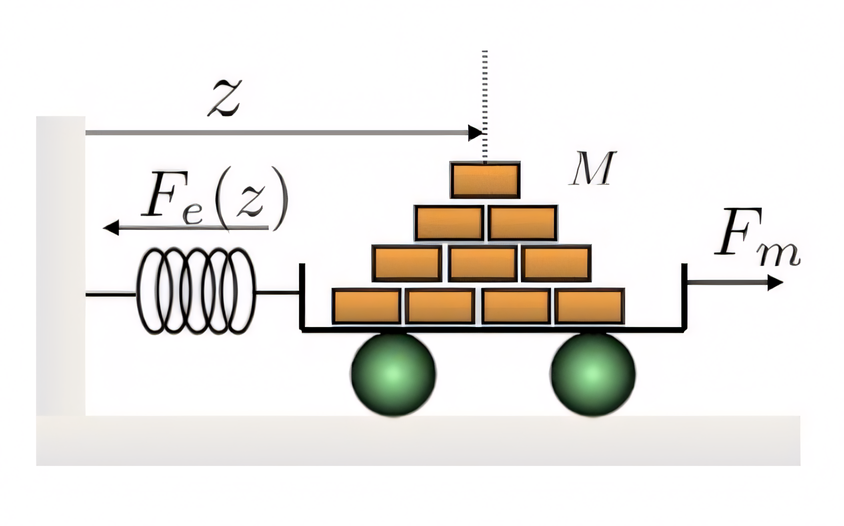
\includegraphics[scale=0.2]{Images/Es_carrello.png}
\end{center}
La legge che usiamo è la legge di Newton, prendendo $z$ come posizione del centro di massa
\begin{equation}
    M \ddot  z = -F_e + F_m
\end{equation}
con $M$ massa e $F_e$ data da
\begin{equation}
    F_e (z(t), t) = k(t)z(t)
\end{equation}
quindi la nostra equazione diventa
\begin{equation}
    M \ddot  z(t) = -k(t)z(t) + F_m(t)
\end{equation}
Siccome nella nostra formula compare una derivata seconda di una variabile ci conviene definire lo stato del sistema con la variabile stessa e la derivata prima della variabile.\\
Definiamo quindi $x_1 := z$ e $x_2:=\dot z$, con stato $x := [x_1x_2]^T$, e $u := F_m$ (ingresso).
\vspace*{0.1cm}\\
Quindi possiamo scrivere, tenendo conto che $\dot x_2(t) = \ddot z$
\begin{align*}
    \dot x_1(t) &= x_2(t)\\
    \dot x_2(t) &= -\frac{k}{M} x_1(t) + \frac{u(t)}{M}
\end{align*}
\begin{equation}
    f(x,u) = 
    \begin{bmatrix}
        f_1(x,u)\\
        f_2(x,u)
    \end{bmatrix}
    :=
    \begin{bmatrix}
        x_2\\
        -\dfrac{k}{M}x_1+\dfrac{u}{M}
    \end{bmatrix}
\end{equation}
Supponiamo di misurare $z(t)$ (sensore posizione), allora $y := z$
\begin{align*}
    \dot x_1(t) &= x_2(t)\\
    \dot x_2(t) &= -\frac{k}{M} x_1(t) + \frac{u(t)}{M}\\
    y(t) &= x_1(t)
\end{align*}
Sia $k(t) = k$ e, ricordando la formula dell'energia cinetica $E_{k}={\dfrac {1}{2}}mv^{2}$ e la formula dell'energia elastica $U={\dfrac {1}{2}}k\,\Delta x^{2}$, consideriamo come uscita l'energia totale $E_T (t) = \dfrac{1}{2} (k z^2 (t) + M \dot z^2 (t))$
\begin{align*}
    \dot x_1(t) &= x_2(t)\\
    \dot x_2(t) &= -\frac{k}{M} x_1(t) + \frac{u(t)}{M}\\
    y(t) &= \frac{1}{2} \left(k(t) x_1^2 (t) + M  x_2^2 (t)\right)
\end{align*}
quindi $h(x):= \dfrac{1}{2} (kx_1^2 + Mx_2^2)$.\\
\textbf{N.B.} Il risultato (l'uscita) vale, di solito, solo per il mio modello, in base a come l'ho impostato; nella realtà potrebbe essere diverso.


\subsection{Esempio auto in rettilineo}
\begin{center}
    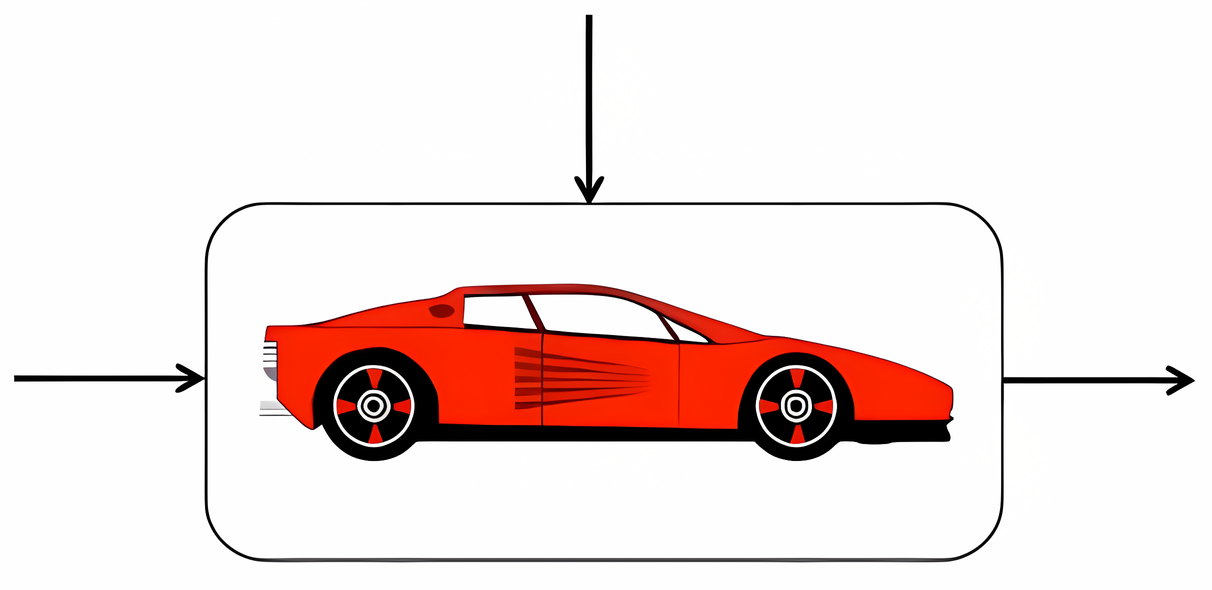
\includegraphics[scale=0.18]{Images/Es_Rettilineo.png}
\end{center}
Scriviamo la legge di Newton
\begin{equation}
    M \ddot z = F_{\text{drag}} + F_m
\end{equation}
con $M$ massa e $F_{\text{drag}}$ data da
\begin{equation}
    F_{\text{drag}} = -b \dot z
\end{equation}
Definiamo $x_1 := z$ e $x_2 := \dot z$ (stato $x := [x_1 x_2 ]^T$ ) e $u := F_m$ (ingresso). Supponiamo di misurare $z(t)$ (sensore posizione), allora $y := z$
\begin{align*}
    \dot x_1(t) &= x_2(t)\\
    \dot x_2(t) &= - \frac{b}{M} x_2(t) + \frac{1}{M}u(t)\\
    y(t) &= x_1(t)
\end{align*}
Proviamo a progettare un sistema per il \textit{cruise control}.\\
L'equazione della dinamica è
\begin{equation}
    M \ddot z(t) = -b\dot z(t) + F_m (t)
\end{equation}
Siccome siamo interessati a controllare la velocità e non la posizione, allora consideriamo come stato solo la velocità: $x := \dot z$, $u := F_m$. Supponiamo di misurare $\dot z(t)$ (sensore velocità), allora $y := x$
\begin{align*}
    \dot x(t) &= - \frac{b}{M}x(t) + \frac{1}{M}u(t)\\
    y(t) &= x(t)
\end{align*}



\subsection{Esempio pendolo}
\begin{center}
    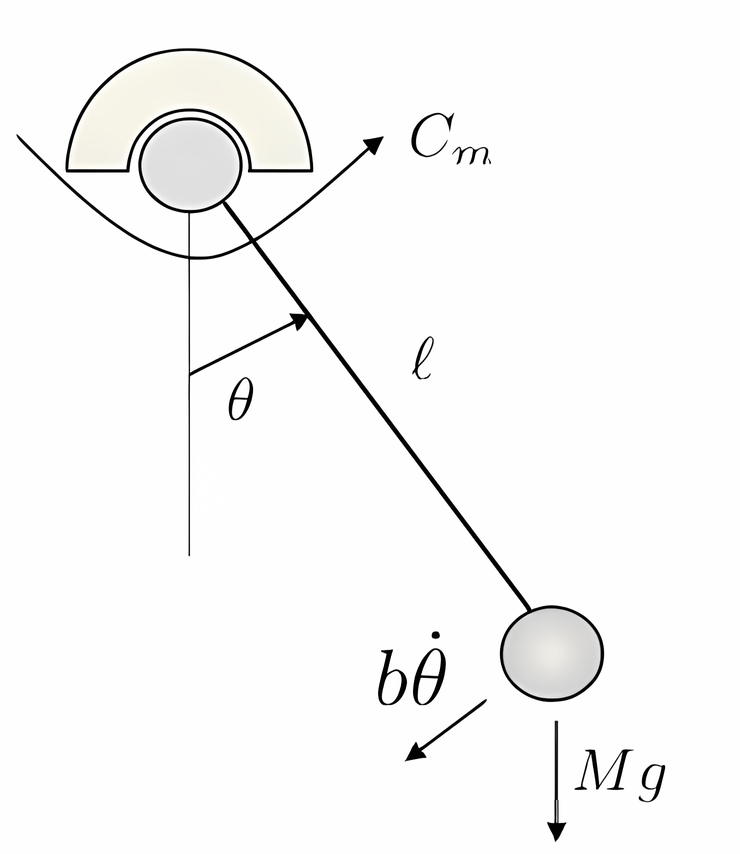
\includegraphics[scale=0.17]{Images/Es_pendolo.png}
\end{center}
Scriviamo l'equazione dei momenti
\begin{equation}
    M \ell^2 \ddot \theta= C_{\T{grav}} + C_{\T{drag}} + C_m
\end{equation}
con $M$ massa e $C_{\T{grav}}$ e $C_{\T{drag}}$ date da
\begin{align*}
    C_{\T{grav}} &=M g \ell \sin(\theta) &
    C_{\T{drag}} &= -b \dot \theta
\end{align*}
con $b$ coefficiente d'attrito.
\vspace*{0.2cm}\\
Scriviamo l'equazione della dinamica, partendo dalla formula iniziale dei momenti

\begin{equation}
    \ddot \theta(t) = -\frac{g}{\ell} \sin \left(\theta(t)\right) - \frac{b}{M \ell^2} \dot \theta(t) + \frac{1}{M \ell^2} C_m(t)
\end{equation}
Definiamo quindi $x_1 := \theta$ e $x_2 := \dot \theta$ (stato $x:= [x_1x_2]^T$) e $u := C_m$ (ingresso).\\
Supponiamo di misurare $\theta$ (sensore angolo) , allora $y := \theta$
\begin{align*}
    \dot x_1 (t) &= x_2(t)\\
    \dot x_2(t) &= -\frac{g}{\ell} \sin \left(x_1(t)\right) - \frac{b}{M \ell^2} x_2(t) + \frac{1}{M \ell^2} u(t)\\
    y(t) &= x_1(t)
\end{align*}
Se misuriamo invece la posizione verticale, allora $y := - \ell \cos(\theta)$ 
\begin{align*}
    \dot x_1 (t) &= x_2(t)\\
    \dot x_2(t) &= -\frac{g}{\ell} \sin \left(x_1(t)\right) - \frac{b}{M \ell^2} x_2(t) + \frac{1}{M \ell^2} u(t)\\
    y(t) &= - \ell \cos(\theta)
\end{align*}



\subsection{Traiettoria di un sistema}
Dato un istante iniziale $t_0$ e uno stato iniziale $x_{t_0}$, la funzione del tempo $(x(t), u(t)), \ t>t_0$, che soddisfa l'equazione di stato $\dot x(t) = f (x(t), u(t), t)$ si dice traiettoria (movimento) del sistema. In particolare, $x(t)$ si dice traiettoria dello stato. Consistentemente, $y(t)$ si dice traiettoria dell'uscita.
\vspace*{0.2cm}\\
\textbf{N.B.} per sistemi senza ingresso (quindi non forzati) la traiettoria dello stato $x(t), \ t>t_0$ è determinata solo dallo stato iniziale $x_{t_0}$.


\subsubsection{Esempio}
Definiamo un sistema con stato $x$ e stato iniziale $x_0$
\begin{align*}
    x &:=
    \begin{bmatrix}
        x_1\\
        x_2
    \end{bmatrix}
    &
    x_0 &:=
    \begin{bmatrix}
        5\\
        3
    \end{bmatrix}
    &
    t_0 &= 0
\end{align*}
\begin{align*}
    \dot x_1(t) &= x_2(t)\\
    \dot x_2(t) &= u(t)
\end{align*}
Assegno a $x_1$, $x_2$ e $u(t)$ le seguenti equazioni
\begin{align*}
    \overline{x_1}(t) &= 5+3t+t^2\\
    \overline{x_2}(t) &= 3+2t\\
    \overline{u}(t) &= 2
\end{align*}
Se le equazioni di $\overline{x_1}$ e $\overline{x_2}$ soddisfano le condizioni iniziali e la funzione di stato ($\dot x_1$ e $\dot x_2$) allora quelle equazioni sono la traiettoria del sistema.\\
Infatti
\begin{equation}
    \overline{x_0} = 
    \begin{bmatrix}
        5+3t+t^2\\
        3+2t
    \end{bmatrix}_{t=0} 
    =
    \begin{bmatrix}
        5\\
        3
    \end{bmatrix}
\end{equation}
\begin{align*}
    &\overline{x_0} = 
    \begin{bmatrix}
        5+3t+t^2\\
        3+2t
    \end{bmatrix}_{t=0} 
    =
    \begin{bmatrix}
        5\\
        3
    \end{bmatrix}
    &
    \frac{d}{dt} 
    \begin{bmatrix}
        5+3t+t^2\\
        3+2t
    \end{bmatrix}
    =
    \begin{bmatrix}
        3+2t\\
        2
    \end{bmatrix}
\end{align*}



\subsection{Equilibrio di un sistema}
Dato un sistema (non forzato) $\dot x(t) = f (x(t), t)$, uno stato $x_e$ si dice \textit{equilibrio del sistema} se $x(t) = x_e$ , $t\geq t_0$ è una traiettoria del sistema.
\vspace*{0.2cm}\\
Dato un sistema (forzato) $\dot x(t) = f (x(t), u(t), t)$, $(x_e , u_e )$ si dice \textit{coppia di equilibrio} del sistema se $(x(t), u(t)) = (x_e , u_e )$, $t \geq t_0$ , è una traiettoria del sistema.
\vspace*{0.2cm}\\
Per un sistema (tempo invariante continuo) $\dot x(t) = f (x(t), u(t))$ data una coppia di equilibrio $(x_e,u_e)$ vale $f(x_e,u_e)=0$.\\
Se il sistema è non forzato, dato un equilibrio $x_e$ vale $f(x_e)=0$.


\subsubsection{Esempio pendolo}
\begin{align*}
    \dot x_1(t) &= x_2(t) &= f_1(x(t),u(t))\\
    \dot x_2(t) &= - \frac{G}{\ell} \sin (x_1(t)) - \frac{b}{M \ell ^2}x_2(t) + \frac{1}{M\ell^2}u(t) &=f_2(x(t),u(t))
\end{align*}
Siccome sappiamo che, data una coppia di equilibrio $(x_e,u_e)$, vale $f(x_e,u_e)=0$, allora per trovare l'equilibrio del pendolo imponiamo 
\begin{equation}
    f(x_e,u_e)=0
\end{equation}
cioè:
\begin{equation}
    \begin{cases}
        x_{2e}(t) = 0\\
        \\
        - \dfrac{G}{\ell} \sin (x_{1e}) - \dfrac{b x_{2e}}{M \ell ^2} + \dfrac{1}{M\ell^2}u_e =0
    \end{cases}
\end{equation}
sostituendo $x_{2e}(t)=0$ nell'ultima equazione
\begin{equation}
    - \dfrac{G}{\ell} \sin (x_{1e}) + \dfrac{1}{M\ell^2}u_e =0 \Longrightarrow u_e = M G \ell \sin(x_{1e})
\end{equation}
In conclusione, le coppie di equilibrio del sistemo sono tutti fli $(x_{1e}, x_{2e},u_e)$ che soddisfano
\begin{equation}
    \begin{cases}
        u_e = M G \ell \sin(x_{1e})\\
        x_{2e}=0
    \end{cases}
\end{equation}




\subsection{Classificazione dei sistemi in forma di stato}
La classe generale è  $x \in \mathbb{R}^n , u \in \mathbb{R}^m , y\in \mathbb{R}^p$
\begin{align*}
    \dot x(t) &= f (x(t), u(t), t) & &\T{equazione di stato}\\
    y(t) &= h(x(t), u(t), t) & &\T{equazione di uscita}  
\end{align*}
\begin{itemize}
    \item I sistemi \textbf{monovariabili} (SISO, Single Input Single Output) sono una sottoclasse di sistemi \textbf{multivariabili} (MIMO, Multiple Input Multiple Output); sono tali se $m=p=1$, altrimenti sono dei sistemi MIMO;
    \item I sistemi \textbf{strettamente propri} sono una sotto classe dei \textbf{sistemi propri}; sono tali se $y(t) = h(x(t),t))$, quindi se l'uscita dipende esclusivamente dall'ingresso, chiamati quindi sistemi causali (tutti i sistemi che abbiamo visto fin'ora sono sistemi propri).
    \item I sistemi \textbf{non forzati} sono una sotto classe dei \textbf{sistemi forzati}; un esempio di sistema non forzato è il seguente
    \begin{align*}
        \dot x(t) &= f(x(t),t)\\
        y(t) &= h(x(t),t)
    \end{align*}
    \item I sistemi \textbf{tempo invarianti} sono una sotto classe di sistemi \textbf{tempo  varianti}.\\
    I tempo invarianti sono tali se, data una traiettoria $ (x(t), u(t)), t\geq t_0$, con $x(t_0)=x_0$, per ogni $\Delta \in \mathbb{R}$ vale che $x(t_0+\Delta)=x_0$ allora $(x_{\Delta} (t), u_{\Delta} (t)) = (x(t-\Delta), u(t-\Delta))$ è una traiettoria.\\
    Si può dimostrare che sistemi tempo invarianti sono del tipo
    \begin{align*}
        \dot x(t) &= f (x(t), u(t)) &x(0)=x_0\\
        y(t) &= h(x(t), u(t))
    \end{align*}
    e senza senza perdita di generalità possiamo scegliere $t_0=0$.\\
    Graficamente:
    \begin{center}
        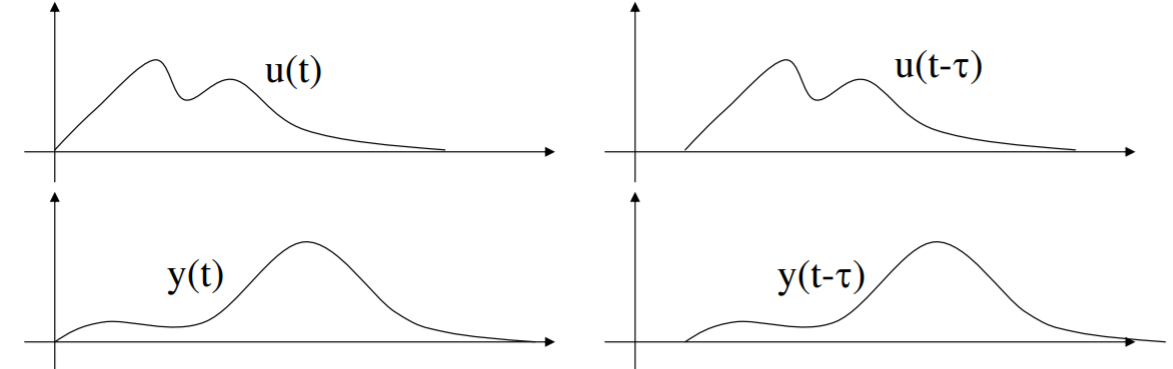
\includegraphics[scale=0.3]{Images/Sistemi_tempo_invarianti.png}
    \end{center}
    \item I \textbf{sistemi lineari} sono una sotto classe di \textbf{sistemi non lineari}.\\
    I sistemi lineari sono tali se le funzioni di stato e di uscita sono lineari in $x$ e $u$:
    \begin{align*}
        \dot x_1 (t) &= a_{11} (t)x_1 (t) + a_{12} (t)x_2 (t) + . . . + a_{1n} (t)x_n (t)+ b_{11} (t)u_1 (t) + b_{12} (t)u_2 (t) + . . . + b_{1m} (t)u_m (t)\\
        \dot x_2 (t) &= a_{21} (t)x_1 (t) + a_{22} (t)x_2 (t) + . . . + a_{2n} (t)x_n (t)+ b_{21} (t)u_1 (t) + b_{22} (t)u_2 (t) + . . . + b_{2m} (t)u_m (t)\\
        ...\\
        ...\\
        ...\\
        \dot x_n (t) &= a_{n1} (t)x_1 (t) + a_{n2} (t)x_2 (t) + . . . + a_{nn} (t)x_n (t)+ b_{n1} (t)u_1 (t) + b_{n2} (t)u_2 (t) + . . . + b_{nm} (t)u_m (t)
    \end{align*}
    per $y(t)$ invece 
    \begin{align*}
        y_1 (t) &= c_{11} (t)x1 (t) + c_{12} (t)x_2 (t) + . . . + c_{1n} (t)x_n (t)+ d_{11} (t)u_1 (t) + d_{12} (t)u_2 (t) + . . . + d_{1m} (t)u_m (t)\\
        y_2 (t) &= c_{21} (t)x_1 (t) + c_{22} (t)x_2 (t) + . . . + c_{2n} (t)x_n (t)+ d_{21} (t)u_1 (t) + d_{22} (t)u_2 (t) + . . . + d_{2m} (t)u_m (t)\\
        ...\\
        ...\\
        ...\\
        y_p (t) &= c_{p1} (t)x_1 (t) + c_{p2} (t)x_2 (t) + . . . + c_{pn} (t)x_n (t)+ d_{p1}(t)u_1 (t) + d_{p2} (t)u_2 (t) + . . . + d_{pm} (t)u_m (t)
    \end{align*}
\end{itemize}



\subsection{Proprietà dei sistemi lineari}
\subsubsection{Sistemi lineri in forma matriciale}
Definiamo le matrici $A(t) \in \mathbb{R}^{n \times n} , B(t) \in \mathbb{R}^{n \times m} , C(t) \in \mathbb{R}^{p \times n} , D(t) \in \mathbb{R}^{p \times m}$
\begin{align*}
    A(t) &= \begin{bmatrix}
        a_{11}(t) & ... & a_{1n}(t)\\
        .\\
        .\\
        a_{n1}(t) & ... & a_{nn}(t)
    \end{bmatrix}
    &
    B(t) &= \begin{bmatrix}
        b_{11}(t) & ... & b_{1m}(t)\\
        .\\
        .\\
        b_{n1}(t) & ... & b_{nm}(t)
    \end{bmatrix}\\
    C(t) &= \begin{bmatrix}
        c_{11}(t) & ... & c_{1n}(t)\\
        .\\
        .\\
        c_{p1}(t) & ... & c_{pn}(t)
    \end{bmatrix}
    &
    D(t) &= \begin{bmatrix}
        d_{11}(t) & ... & d_{1m}(t)\\
        .\\
        .\\
        d_{pn1}(t) & ... & d_{pm}(t)
    \end{bmatrix}
\end{align*}
quindi scriviamo
\begin{equation}
    \begin{bmatrix}
        \dot x_1(t)\\
        .\\
        .\\
        \dot x_n(t)
    \end{bmatrix}
    = A(t)
    \begin{bmatrix}
        x_1(t)\\
        .\\
        .\\
        x_n(t)
    \end{bmatrix}
    + B(t)
    \begin{bmatrix}
        u_1(t)\\
        .\\
        .\\
        u_m(t)
    \end{bmatrix}
\end{equation}
che equivale a 
\begin{align*}
    \dot x(t) &= A(t) x(t) + B(t) u(t)\\
    y(t) &= C(t)x(t) + D(t) u(t)
\end{align*}


\subsection{Sistemi lineari tempo-invarianti}
\begin{align*}
    \dot x(t) = A x(t) + B u(t)\\
    y(t) = C x(t) + D u(t)
\end{align*}
con $A,B,C,D$ matrici costanti.


\subsubsection{Esempio carrello}
\begin{center}
    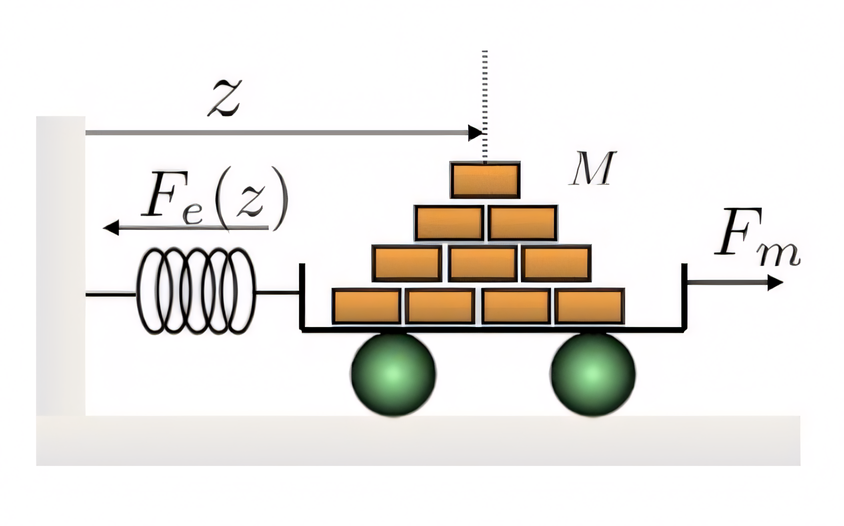
\includegraphics[scale=0.2]{Images/Es_carrello.png}
\end{center}
\begin{align*}
    \dot x_1(t) &= x_2(t) & f_1(x,u,t) &= x_2\\
    \dot x_2(t) &= - \frac{k(t)}{M}x_1(t) + \frac{1}{M} u(t) & f_2(x,u,t) &= - \frac{k(t)}{M}x_1 + \frac{1}{M}u\\
    y(t) &= x_1(t)
\end{align*}
$f_2$ dipende esplicitamente da $t$ attraverso $k(t)$ quindi è un sistema tempo \underline{variante}. Se $k(t) = \overline{k}$ per ogni $t$ allora tempo \underline{invariante}.\\
Siccome $f_1$ e $f_2$ dipendono linearmente da $x$ e $u$ il sistema è \underline{lineare}. (Se $k(t) = \overline{k}$ il sistema è \underline{lineare tempo invariante}.)
\begin{align*}
    \begin{bmatrix}
        \dot x_1(t)\\
        \dot x_2(t)
    \end{bmatrix}
    &=
    \underbrace{\begin{bmatrix}
        0 & 1\\
        -\frac{k(t)}{M} & 0
    \end{bmatrix}}_{A}
    \begin{bmatrix}
        x_1(t)\\
        x_2(t)
    \end{bmatrix}
    +
    \underbrace{\begin{bmatrix}
        0\\
        \frac{1}{M}
    \end{bmatrix}}_{B}
    u(t)
    \\
    y(t) &= 
    \underbrace{\begin{bmatrix}
        1 & 0
    \end{bmatrix}}_{C}
    \begin{bmatrix}
        x_1(t)\\
        x_2(t)
    \end{bmatrix}
    + \underbrace{0}_D u(t)
\end{align*}
per $k$ costante:
\begin{align*}
    A &= \begin{bmatrix}
        0 & 1\\
        - \frac{k}{M} & 0
    \end{bmatrix}
    &
    B &= 
    \begin{bmatrix}
        0\\
        1
    \end{bmatrix}
    &
    C &= 
    \begin{bmatrix}
        1 & 0
    \end{bmatrix}
\end{align*}


\subsubsection{Sistemi lineari tempo-invarianti SISO}
I sistemi lineari tempo-invarianti single input single output (SISO) sono caratterizzati dalle matrici $A \in \mathbb{R}^{n \times n} , B \in \mathbb{R}^{n \times 1}, C \in \mathbb{R}^{1 \times n} , D \in \mathbb{R}^{1 \times 1}$, ovvero $B$ è un vettore, $C$ è un vettore riga e $D$ è uno scalare.


\subsection{Principio di sovrapposizione degli effetti}
Prendiamo un sistema lineare (anche tempo-variante)
\begin{align*}
    \dot x(t) &= A(t)x(t) + B(t)u(t)\\
    y(t) &= C(t)x(t) + D(t)u(t)
\end{align*}
Sia $(x_a (t), u_a (t))$ traiettoria con $x_a (t_0)$ = $x_{0a}$.\\
Sia $(x_b (t), u_b (t))$ traiettoria con $x_b (t_0)$ = $x_{0b}$.
\vspace*{0.1cm}\\
Allora $\forall \alpha, \beta \in \mathbb{R}$ dato lo stato iniziale $x_{ab}(t_0) = \alpha x_{0a}+\beta x_{0b}$, si ha che
\begin{equation}
    (x_{ab}(t), u_{ab}(t)) = (\alpha x_{a}(t) + \beta x_b(t), \alpha u_a(t)+\beta u_b(t))
\end{equation}
è traiettoria del sistema, ovvero applicando come ingresso $u_{ab}=\alpha u_a(t) + \beta u_b(t)$ la traiettoria di stato è $x_{ab} (t) = \alpha x_a (t) + \beta x_b (t)$
\begin{equation}
    \begin{rcases}
        \alpha x_{0a}(t)+\beta x_{0b}(t)\\
        \alpha u_a(t) + \beta u_b(t)(t)
    \end{rcases}
    \Longrightarrow
    \alpha x_a(t) + \beta x_b(t)
\end{equation}
\vspace*{0.2cm}
\textbf{IMPORTANTE:} non vale per i sistemi non lineari.

\subsubsection*{Dimostrazione}
Per dimostrarlo dobbiamo provare che soddisfa l'equazione differenziale
\begin{align*}
    \frac{d}{dt}x_{ab}(t) &= \alpha \dot x_a(t) + \beta \dot x_b(t)\\
    &= \alpha(A(t)x_a (t) + B(t)u_a (t)) + \beta (A(t)x_b (t) + B(t)u_b (t))\\
    &= A(t)(\alpha x_a (t) + \beta x_b (t)) + B(t)( \alpha u_a (t) + u_b (t))
\end{align*}
Per sistemi lineari sotto opportune ipotesi su $A(t)$ e $B(t)$ si può dimostrare che la soluzione è unica.\\
Si dimostra lo stesso anche per l'uscita.


\subsection{Evoluzione libera e evoluzione forzata}
Sfruttando il principio di sovrapposizione degli effetti prendiamo due sistemi \circled{A} e \circled{B} 
\begin{align*}
   \circled{A} \ x(t_0) &= x_0 =x_{0a} {\color{violet} \neq 0} & \circled{B} \ \ \ x_{0b}&=0\\
    u_a(t) &= 0 \ \ \forall t \geq t_0 & u_b(t) &= u(t) {\color{violet}\neq 0}
\end{align*}
chiamiamo $x_a(t)=x_\ell(t)$ e $x_b(t) = x_f(t)$
\begin{align*}
    \alpha x_{0a} + \beta x_{0b} &= \underbrace{\alpha}_{1} x_0 = x_0 & 
    \alpha u_a(t) + \beta u_b(t) &= \underbrace{\beta}_{1}u(t) = u(t)
\end{align*}
quindi
\begin{equation}
    x_{ab}(t) = \underbrace{x_\ell(t)}_{\substack{\text{evoluzione} \\ \text{libera}}} + \underbrace{x_f(t)}_{\substack{\text{evoluzione} \\ \text{forzata}}}
\end{equation}
L'\textbf{evoluzione libera} è definita come $x_\ell(t)$ per $t \geq t_0$, tale che $x_\ell (t_0)=x_0$ e $u_l(t)=0$ per $t \geq t_0$, e uscita $y_\ell(t)=C(t)x_\ell(t)$.\\
L'\textbf{evoluzione forzata} è definita come $x_f(t)$ per $t \geq t_0$, tale che $x_f (t_0)=0$ e $u_l(t)=u(t)$ per $t \geq t_0$, e uscita $y_f(t)=C(t)x_f(t)+D(t)u(t)$.
\vspace*{0.2cm}\\
\textbf{IMPORTANTE:} non vale per i sistemi non lineari.


\subsubsection{Traiettorie di un sistema LTI: esempio scalare}
Definiamo un sistema lineare tempo invariante (LTI) scalare $x \in \mathbb{R}$, $u \in \mathbb{R}$, $y \in \mathbb{R}$
\begin{align*}
    \dot x(t) &= ax(t) + bu(t) &x(0) = x_0\\
    y(t) &= cx(t) + du(t)
\end{align*}
dall'analisi matematica possiamo scrivere il sistema come soluzione omogenea + soluzione particolare
\begin{align*}
    x(t) &= e^{at}x_0 + \int_0^t e^{a(t-\tau)}bu(\tau) d \tau \\
    y(t) &= ce^{at}x_0 + c \int_0^t e^{a(t-\tau)}bu(\tau) d \tau + du(t)
\end{align*}
ricordiamo che la funzione esponenziale si può scrivere come
\begin{equation}
    e^{at} = 1 + at + \frac{(at)^2}{2!} + \frac{(at)^3}{3!} + ...
\end{equation}


\subsubsection{Traiettorie di un sistema LTI: caso generale}
Definiamo un sistema lineare tempo invariante (LTI) $x\in \mathbb{R}^n, u\in \mathbb{R}^m, y\in \mathbb{R}^p$
\begin{align*}
    \dot x(t) &= Ax(t) + Bu(t) &x(0) = x_0\\
    y(t) &= Cx(t) + Du(t)
\end{align*}
\begin{align*}
    \underbrace{x(t)}_{\mathbb{R}^n} &= \underbrace{e^{At}}_{\mathbb{R}^{n \times n}} \underbrace{x_0}_{\mathbb{R}^n} + \int_0^t e^{A(t-\tau)}Bu(\tau) d \tau \\
    y(t) &= Ce^{at}x_0 + c \int_0^t e^{A(t-\tau)}Bu(\tau) d \tau + Du(t)
\end{align*}

Ricordiamo che l'esponenziale di matrice si può scrivere come
\begin{equation}
    e^{At} = I + At + \frac{(At)^2}{2!} + \frac{(At)^3}{3!} + ...
\end{equation}
\begin{equation}
    x(t) = \underbrace{e^{At} x_0}_{\substack{\text{evoluzione} \\ \text{libera}}} + \underbrace{\int_0^t e^{A(t-\tau)}Bu(\tau) d \tau}_{\substack{\text{evoluzione} \\ \text{forzata}}}
\end{equation}
\begin{align*}
    x_\ell(t) &= e^{At}x_0 & x_f(t) &= \int_0^t e^{A(t-\tau)}Bu(\tau) d \tau
\end{align*}


\subsubsection{Esempio sistema non forzato}
\begin{align*}
    \dot x_1(t) = \lambda_1 x_1(t) & \dot x_1(t) = \lambda_2 x_2(t)
\end{align*}
\begin{equation}
    \begin{bmatrix}
        \dot x_1(t)\\
        \dot x_2(t)
    \end{bmatrix}
    =
    \underbrace{\begin{bmatrix}
        \lambda_1 & 0\\
        0 & \lambda_2  
    \end{bmatrix}}_{A}
    \begin{bmatrix}
        x_1(t)\\
        x_2(t)
    \end{bmatrix}
\end{equation}
$A := \Lambda$ matrice diagonale.
\vspace*{0.2cm}\\
Il nostro è un sistema non forzato, quindi c'è solo l'evoluzione libera:
\begin{equation}
    x(t) = e^{\Lambda t}x_0
\end{equation}
\begin{align*}
    e^{\Lambda t} &= 
    \begin{bmatrix}
        1 & 0\\
        0 & 1
    \end{bmatrix}
    +
    \begin{bmatrix}
        \lambda_1 & 0\\
        0 & \lambda_2
    \end{bmatrix}
    +
    \begin{bmatrix}
        \lambda_1 & 0\\
        0 & \lambda_2
    \end{bmatrix}^2 \frac{t^2}{2!} + ...\\
    &=\begin{bmatrix}
        1 & 0\\
        0 & 1
    \end{bmatrix}
    +
    \begin{bmatrix}
        \lambda_1 & 0\\
        0 & \lambda_2
    \end{bmatrix}
    +
    \begin{bmatrix}
        \frac{\lambda_1^2 t^2}{2!} & 0\\
        0 & \frac{\lambda_2^2 t^2}{2!}
    \end{bmatrix} + ...\\
    e^{at} = 1 + at + \frac{(at)^2}{2!} + \frac{(at)^3}{3!} + ... \Longrightarrow&=
    \begin{bmatrix}
        e^{\lambda_1 t} & 0\\
        0 & e^{\lambda_2 t}
    \end{bmatrix}
\end{align*}
Quindi nel caso generale di $\Lambda \in \mathbb{R}^{n \times n}$
\begin{equation}
    e^{\Lambda t} = 
    \begin{bmatrix}
        e^{\lambda_1 t} & 0 & ... & 0\\
        0 & e^{\lambda_2 t} & ... & 0\\
        .\\
        .\\
        0 & ... & 0 & e^{\lambda_n t}
    \end{bmatrix}
\end{equation}


\subsubsection{Proprietà della matrice esponenziale} \label{proprietà della matrice esponenziale}
Esponenziale e cambio di base:
\begin{equation}
    e^{TAT^{-1}} = Te^{At}T^{-1}
\end{equation}
Data una matrice $A \in \mathbb{R}^{n \times n}$, esiste $J$ matrice diagonale a blocchi, chiamata \textit{matrice di Jordan}, che è unica a meno di permutazioni dei blocchi, tale che
\begin{equation}
    A = T^{-1} J T
\end{equation}
con $T$ matrice invertibile (matrice del cambio base). Questa formula viene chiamata \textit{forma di Jordan}.
\vspace*{0.2cm}\\
La matrice di Jordan è fatta in questo modo
\begin{center}
    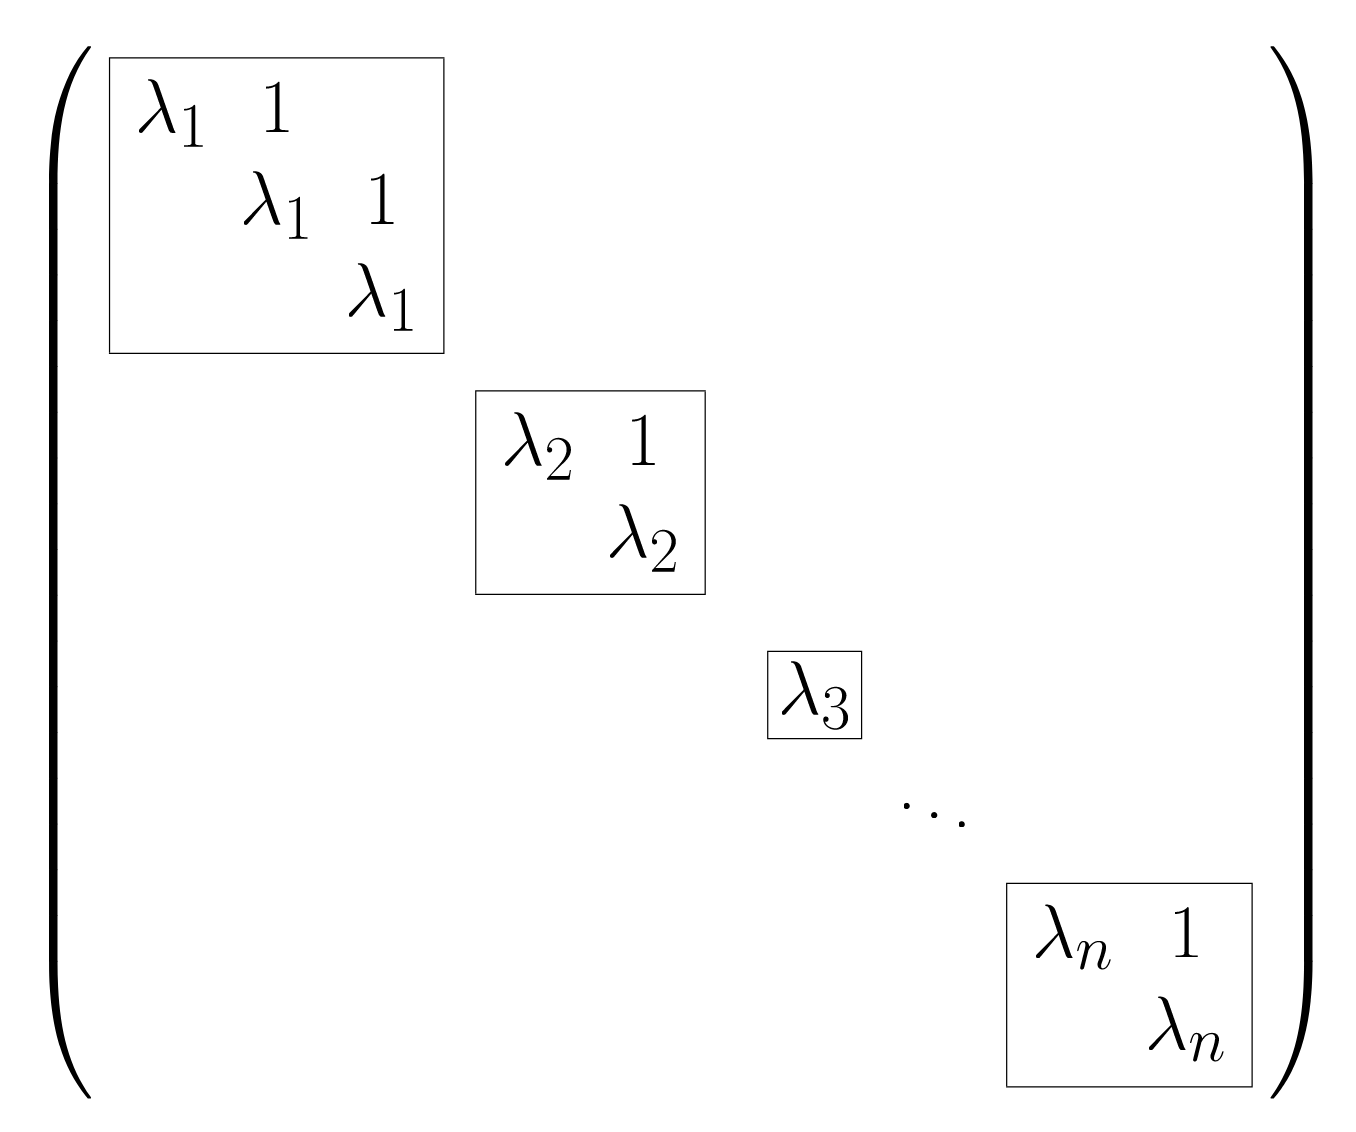
\includegraphics[scale=0.13]{Images/Jordan_matrix.png}
\end{center}
con $\lambda_i$ autovalore di $A$.
\vspace*{0.2cm}\\
Utilizzando questa forma riconduco il calcolo di $e^{At}$ al calcolo di 
\begin{equation}
    e^{
        \begin{bmatrix} 
            \lambda & 1 & 0 & ... & 0\\
            0 & ... & ... & ... &0\\
            ... & ... & ... & ... & 0\\
            ... & ... & ... & ... & 1\\
            0 & ... & ... & 0 & \lambda
        \end{bmatrix}
        }
        = e^{\lambda t}
        \begin{bmatrix}
            1 & t & \frac{t^2}{2!} & ... \\
            0 & 1 & t & \frac{t^2}{2!} & ... \\
            ... & ... & ... & ... & ...\\
            0 & ... & ... & ... & 1
        \end{bmatrix}
\end{equation}
\textbf{IMPORTANTE:} tutti gli elementi di $e^{At}$ sono del tipo
\begin{equation}
    t^qe^{\lambda t}
\end{equation}
con $q$ intero e $\lambda_i$ autovalori di A


\subsection{Rappresentazioni equivalenti}
Effettuiamo un cambio di base mediante una matrice $T$
\begin{equation}
    \hat x(t) = T x(t)
\end{equation}
ed essendo $T$ invertibile
\begin{equation}
    x(t) = T^{-1} \hat x(t)
\end{equation}
Sostituendo nell'equazione della dinamica si ottiene
\begin{align*}
    {\color{violet} T \cdot} \underbrace{T^{-1} \dot{\hat x}(t)}_{\dot x(t)} &= A \underbrace{T^{-1} \hat x(t)}_{x(t)} + B u(t) {\color{violet} \cdot T } \\
\end{align*}
\begin{align*}
    \dot{\hat x}(t) &= TAT^{-1} \hat x(t) + T B u(t)\\
    y(t) &= CT^{-1} \hat x(t) + D u(t)
\end{align*}
Allora chiamo $\hat A = TAT^{-1}, \hat B=TB, \hat C = CT^{-1}, \hat D = D$
\begin{align*}
    \dot{\hat x}(t)  &= \hat A \hat x(t) + \hat B u(t)\\
    y(t) &= \hat C \hat x(t) + \hat D u(t)
\end{align*}
se $T$ è una matrice tale che
\begin{equation}
    J = TAT^{-1}
\end{equation}
allora
\begin{equation}
    \dot{\hat x} = J \hat x(t) + T B u(t)
\end{equation}
\begin{align*}
    \hat x_\ell (t) = e^{JT} \hat x_0 = T^{-1} e^{Jt}T x_0
\end{align*}




\subsection{Modi di un sistema lineare tempo invariante}
Prendiamo un sistema lineare tempo invariante con $x \in \mathbb{R}^n, u \in \mathbb{R}^m, y \in \mathbb{R}^p$ e $x(0)=x_0$
\begin{align*}
    \dot x(t) &= A x(t) + B u(t)\\
    y(t) &= C x(t) + D u(t)
\end{align*}
Indichiamo con $\lambda_1,...,\lambda_r$ gli $r \leq n$ autovalori (reali o complessi coniugati) distinti della matrice $A$, con molteplicità algebrica $n_1,...,n_r \geq 0$ tali che $\sum\limits ^r_{i=1} n_i = n$.\\
Le componenti dell'evoluzione libera dello stato $x_\ell(t)$ si possono scrivere come
\begin{equation}
    x_{\ell,j} = \sum^r_{i=1}\sum^{h_i}_{q=1} \gamma_{jiq}t_{q-1}e^{\lambda_i t} \tag*{$j=1,...,n$}
\end{equation}
per opportuni valori di $h_i \leq n_i$, dove i coefficienti $\gamma_{jiq}$ dipendono dallo stato iniziale $x(0)$.\\
I termini $t^{q-1}e^{\lambda_i t}$  sono detti modi naturali del sistema.
L'evoluzione libera dello stato è combinazione lineare dei modi.


\subsubsection{Autovalori complessi}
Se la matrice $A$ è reale e $\lambda_i = \sigma_i + j \omega_i$ è un autovalore complesso, allora il suo complesso coniugato $\overline{\lambda}_i = \sigma_i - j \omega_i$ è anch'esso autovalore di $A$.\\
Inoltre si dimostra che i coefficienti $\gamma_{jiq}$ corrispondenti a $\lambda_i$ e $\overline{\lambda}_i$ sono anch'essi complessi coniugati.\\
Scriviamo l'\textbf{esponenziale di autovalori complessi coniugati}; se $\lambda_i = \sigma_i + j \omega_i$ e $\overline{\lambda}_i = \sigma_i - j \omega_i$ allora
\begin{align*}
    e^{\lambda_i t} &= e^{\sigma_i + j \omega_i} & e^{\overline{\lambda}_i t} &= e^{\sigma_i - j \omega_i}\\
    &= e^{\sigma_i t} e^{j \omega_i t} & &= e^{\sigma_i t} e^{-j \omega_i t}\\
    &= e^{\sigma_i t} (\cos(\omega_i t) + j \sin(\omega_i t)) & &= e^{\sigma_i t} (\cos(\omega_i t) - j \sin(\omega_i t))
\end{align*}
Si verifica quindi, per calcolo diretto, che le soluzioni $x_{\ell,j}(t)$ sono sempre reali e che i modi del sistema corrispondenti ad autovalori complessi coniugati $\lambda_i$ e $\overline{\lambda}_i$ sono del tipo
\begin{equation}
    t^{q-1} e^{\sigma_i t} \cos (\omega_i t + \phi_i)
\end{equation}
con opportuni valori della fase $\phi_i$.
\vspace*{0.2cm}\\
Supponiamo che le molteplicità algebriche $n_1,...,n_r$ degli autovalori di $A$ coincidano cone le molteplicità geometriche (ad esempio quando gli autovalori sono distinti).\\
Allora i coefficienti $h_i$ sono tutti pari a 1 e l'espressione dei modi si semplifica in 
\begin{align*}
    &e^{\lambda_i t} & &\T{per autovalori reali}\\
    &e^{\sigma _i t} \cos (\omega_i t + \phi_i) & &\T{per autovalori complessi coniugati}
\end{align*}

\subsubsection*{Modi naturali: autovalori reali semplici} \label{Modi naturali: autovalori reali semplici}
\begin{center}
    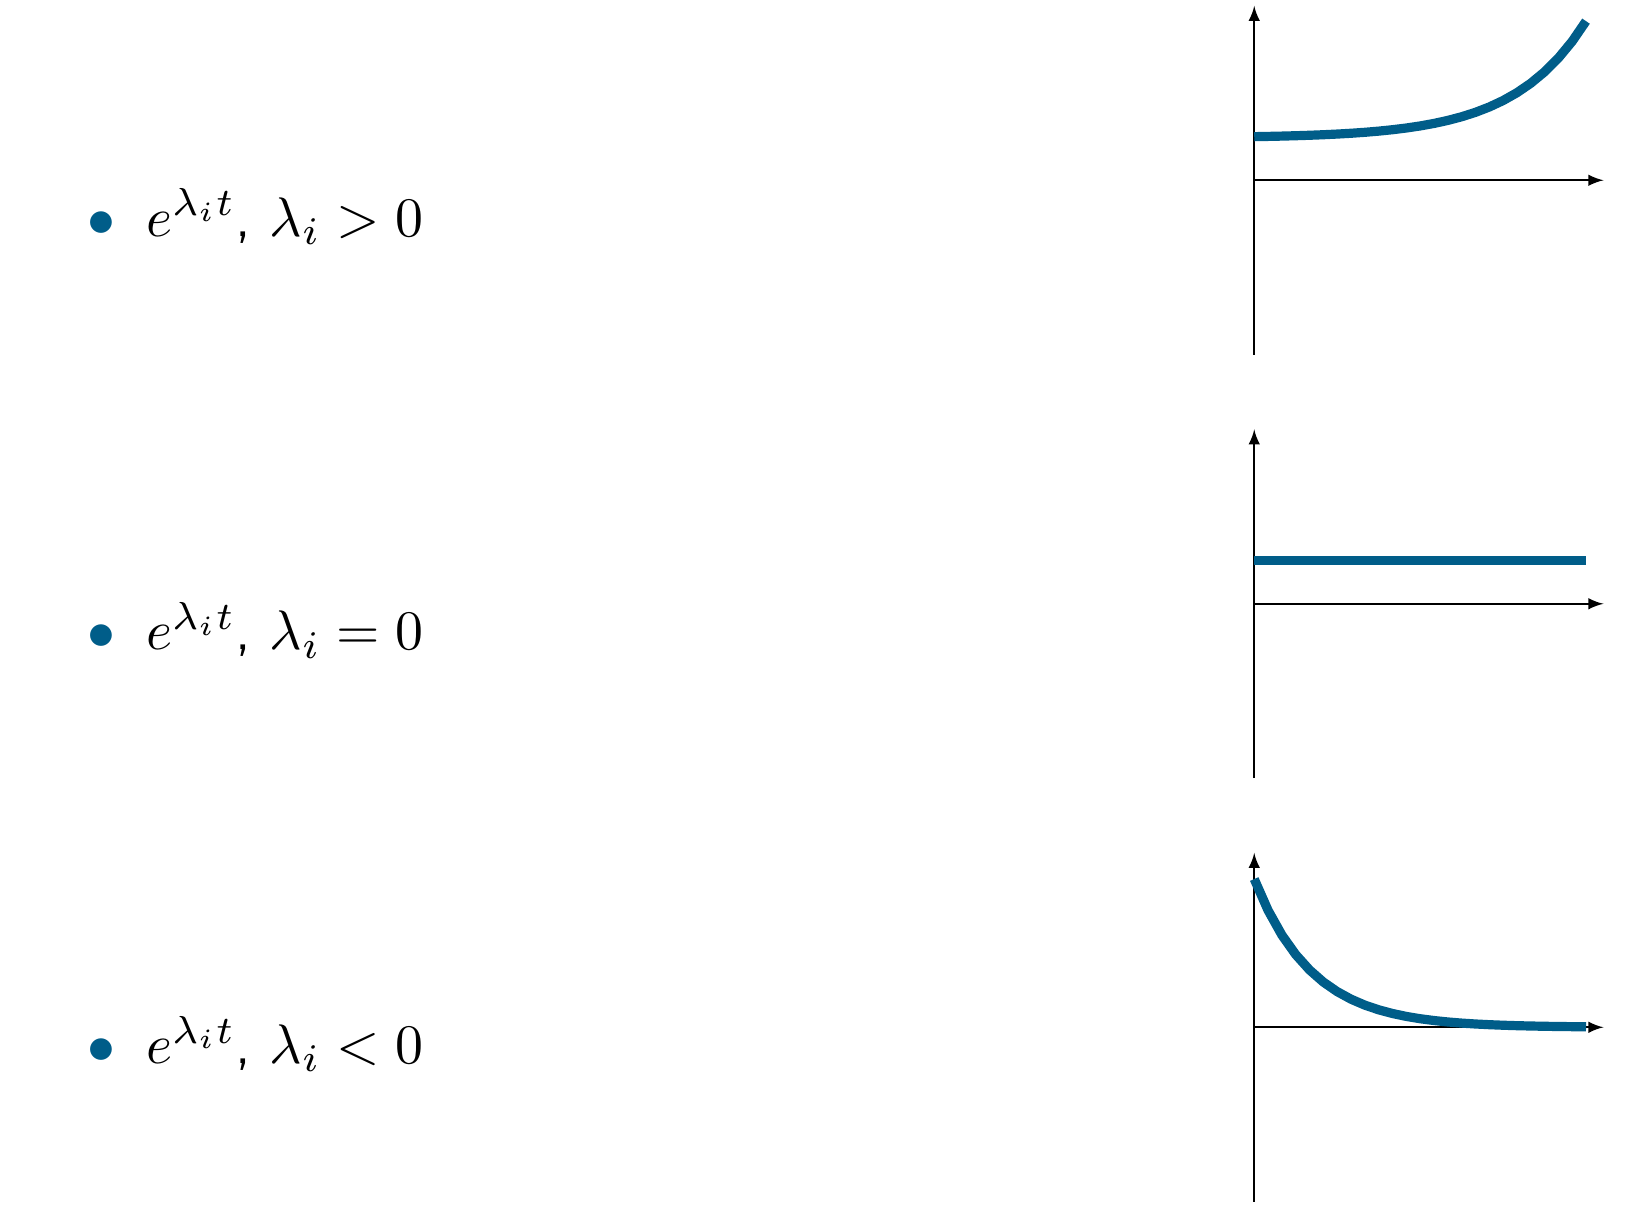
\includegraphics[scale=0.23]{Images/Autovalori_semplici.png}
\end{center}


\subsubsection*{Modi naturali: autovalori complessi coniugati semplici}
\begin{center}
    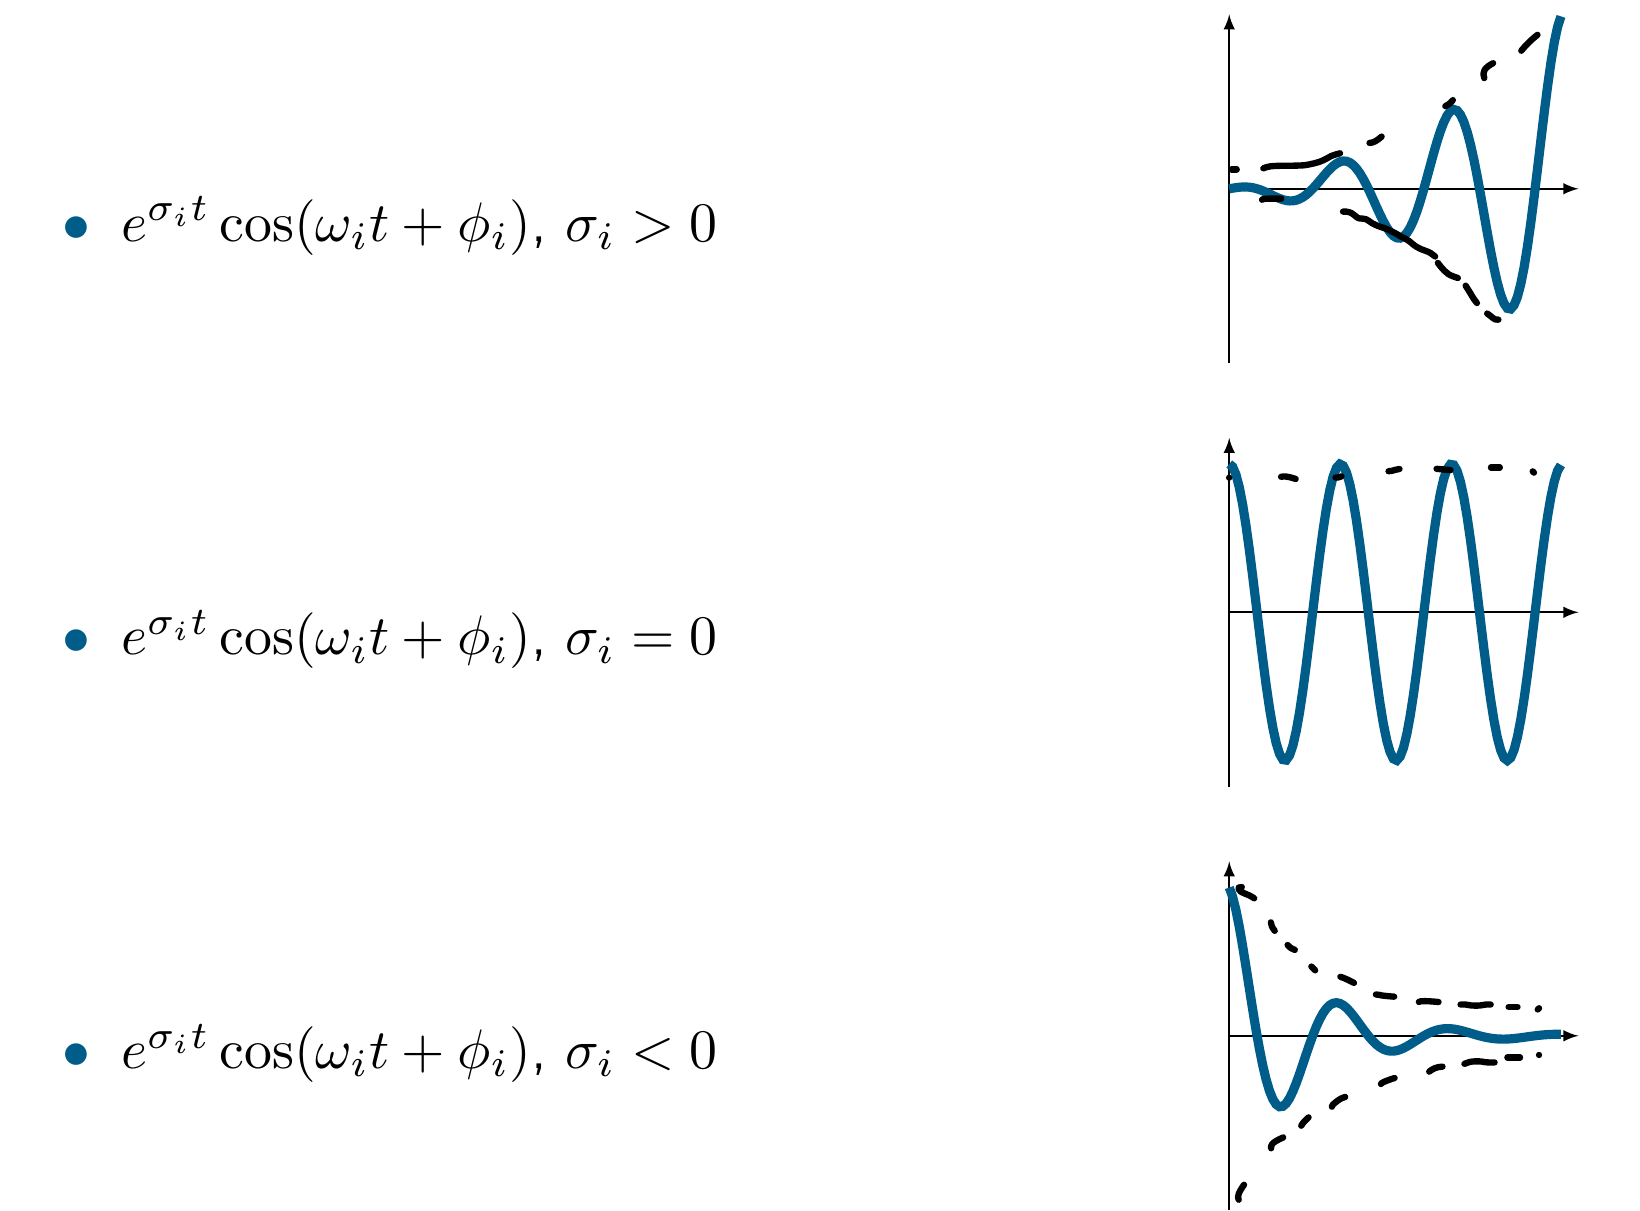
\includegraphics[scale=0.23]{Images/Autovalori_comlessi.png}
\end{center}

\begin{center}
    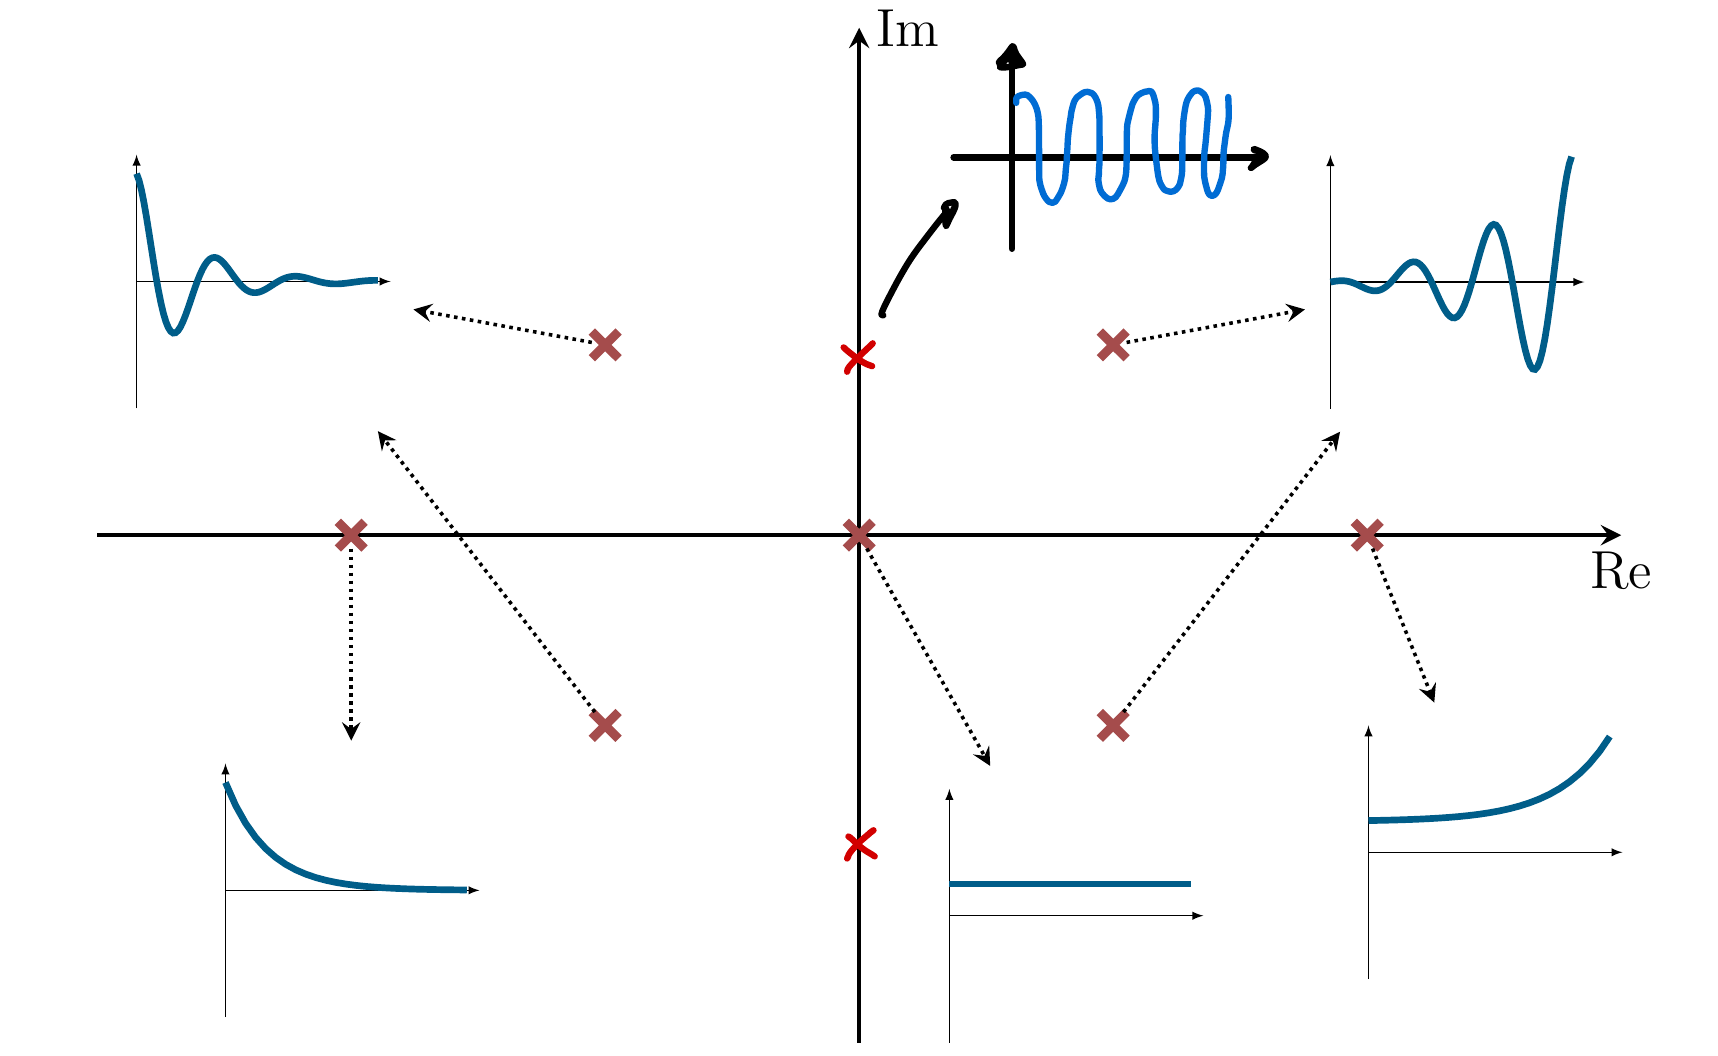
\includegraphics[scale=0.23]{Images/Esempio_autovalori.png}
\end{center}

\subsubsection{Esempio sui modi naturali}
\begin{equation}
    \begin{bmatrix}
        \dot x_1\\
        \dot x_2
    \end{bmatrix}
    =
    \begin{bmatrix}
        0 & 1\\
        a^2 & 0
    \end{bmatrix}
    \begin{bmatrix}
        x_1\\
        x_2
    \end{bmatrix}
\end{equation}

\begin{align*}
    p(\lambda) &= \det (\lambda I -A)\\
    &= \lambda^2 - a^2\\
    &\Rightarrow \begin{cases}
        \lambda_1 = a\\
        \lambda_2 = -a
    \end{cases}
\end{align*}
I modi naturali di questo sistema sono 
\begin{align*}
    &e^{at} & &e^{-at}
\end{align*}
Il modo $e^{at}$ diverge a infinito, il che non è una cosa "buona" per dei sistemi di controllo, perché ad esempio se si sta realizzando un sistema di controllo della velocità vuol dire che la mia velocità sta aumentando, mentre dovrebbe rimanere fissa in un range.\\
Non bisogna quindi focalizzarsi sul calcolare con precisione il valore dei modi naturali ma è importante conoscere come si comporta la loro parte reale.


\subsubsection{Esempio 1}
Consideriamo il seguente sistema LTI con $x \in \mathbb{R}^3 e u \in \mathbb{R}^3$
\begin{equation}
    \dot x(t) = \underbrace{\begin{bmatrix}
        0 & 1 & -1\\
        1 & -1 & -1\\
        2 & 1 & 3 
    \end{bmatrix}}_{A} x(t) +
    \underbrace{\begin{bmatrix}
        1 & 1 & 0\\
        0 & 1 & 1\\
        1 & 1 & 1
    \end{bmatrix}}_{B} u(t)
\end{equation}
Mediante un cambio di coordinate usando la matrice $T = \begin{bmatrix}
    0 & -1 & 1\\ 1 & 1 & -1\\ -1 & 0 & 1
\end{bmatrix}$ e ponendo $\hat x(t) = T x(T)$, il sistema si può riformulare come 
\begin{equation}
    \hat{\dot x} (t)= \underbrace{\begin{bmatrix}
        -1 & 1 & 0\\
        0 & -1 & 0\\
        0 & 0 & -2 
    \end{bmatrix}}_{\hat A = TAT^{-1}} \hat x(t) +
    \underbrace{\begin{bmatrix}
        1 & 0 & 0\\
        0 & 1 & 0\\
        0 & 0 & 1
    \end{bmatrix}}_{\hat B = TB} u(t)
\end{equation}
Gli autovalori di $\hat A$ sono $-1, -2$ con molteplicità algebrica $2,1$.
\vspace*{0.2cm}\\
Per calcolare l'evoluzione libera consideriamo la formula vista in precedenza
\begin{equation}
    \hat x_\ell  =e^{\hat A t}\hat x_0
\end{equation}
Calcoliamo quindi l'esponenziale di matrice $e^{\hat A t}$ per $\hat A = \begin{bmatrix}
    -1 & 1 & 0\\
    0 & -1 & 0\\
    0 & 0 & -2
\end{bmatrix}$
\begin{align*}
    e^{\hat A t} &= \sum_{k=0}^\infty \begin{bmatrix}
        -1 & 1 & 0\\
        0 & -1 & 0\\
        0 & 0 & -2
    \end{bmatrix}^k \frac{t^k}{k!}\\
    &= \begin{bmatrix}
        \sum\limits_{k=0}^\infty \frac{(-1)^k t^k}{k!} & t \sum\limits_{k=0}^\infty \frac{(-1)^k t^k}{k!} & 0\\
        0 & \sum\limits_{k=0}^\infty \frac{(-1)^k t^k}{k!} & 0\\
        0 & 0 & \sum\limits_{k=0}^\infty \frac{(-2)^k t^k}{k!}
    \end{bmatrix}\\
    &= \begin{bmatrix}
        e^{-t} & te^{-t} & 0\\
        0 & e^{-t} & 0\\
        0 & 0 & e^{-2t}
    \end{bmatrix}
\end{align*}
quindi l'evoluzione libera dello stato è
\begin{equation}
    \hat x_\ell = 
    \begin{bmatrix}
        e^{-t} & te^{-t} & 0\\
        0 & e^{-t} & 0\\
        0 & 0 & e^{-2t}
    \end{bmatrix} \hat x_0
\end{equation}
\begin{itemize}
\item Se ad esempio la condizione iniziale è $\hat x_0 = \begin{bmatrix} 1\\0\\0 \end{bmatrix}$, allora
\begin{equation}
    \hat x_\ell = \begin{bmatrix} e^{-t}\\0\\0 \end{bmatrix}
\end{equation}
Scriviamolo nello coordinate originali
\begin{equation}
    x_\ell(t) = \underbrace{\begin{bmatrix}
        1&1&0\\
        0&1&1\\
        1&1&1
    \end{bmatrix}}_{T^{-1}} \hat x_\ell (t) = 
    \begin{bmatrix}
        e^{-t}\\
        0\\
        e^{-t}
    \end{bmatrix}
\end{equation}
\item Se prendiamo come condizione iniziale $\hat x_0 = \begin{bmatrix} 0\\1\\0 \end{bmatrix}$, allora
\begin{equation}
    \hat x_\ell = \begin{bmatrix} te^{-t}\\e^{-t}\\0 \end{bmatrix}
\end{equation}
Scriviamolo nello coordinate originali
\begin{equation}
    x_\ell(t) = \underbrace{\begin{bmatrix}
        1&1&0\\
        0&1&1\\
        1&1&1
    \end{bmatrix} }_{T^{-1}} \hat x_\ell (t) = 
    \begin{bmatrix}
        e^{-t} + te^{-t}\\
        e^{-t}\\
        e^{-t} + te^{-t}
    \end{bmatrix}
\end{equation}


\item Se prendiamo come condizione iniziale $\hat x_0 = \begin{bmatrix} 0\\0\\1 \end{bmatrix}$. allora
\begin{equation}
    \hat x_\ell = \begin{bmatrix} 0\\0\\e^{-2t} \end{bmatrix}
\end{equation}
Nelle coordinate originali:
\begin{equation}
    x_\ell(t) = \underbrace{\begin{bmatrix}
        1&1&0\\
        0&1&1\\
        1&1&1
    \end{bmatrix} }_{T^{-1}} \hat x_\ell (t) = 
    \begin{bmatrix}
        0\\
        e^{-2t}\\
        e^{-2t}
    \end{bmatrix}
\end{equation}

\end{itemize}


\subsubsection{Esempio carrello}
\begin{align*}
    \dot x_1(t) &= x_2(t) \\
    \dot x_2(t) &= - \frac{k(t)}{M}x_1(t) + \frac{1}{M} u(t) \\
    y(t) &= x_1(t)
\end{align*}
\begin{align*}
    \begin{bmatrix}
        \dot x_1(t)\\
        \dot x_2(t)
    \end{bmatrix} &=
    \begin{bmatrix}
        0 & 1\\
        - \frac{k}{M} & 0
    \end{bmatrix}
    \begin{bmatrix}
        x_1(t)\\
        x_2(t)
    \end{bmatrix}
    +
    \begin{bmatrix}
        0\\
        \frac{1}{M}
    \end{bmatrix} u(t)
    \\
    y(t) &= \begin{bmatrix}
        1 & 0
    \end{bmatrix}
    \begin{bmatrix}
        x_1(t)\\
        x_2(t)
    \end{bmatrix} + 0 u(t)
\end{align*}
Consideriamo $k$ costante, quindi sistema LTI.\\
Gli autovalori della matrice $A$ sono $\lambda_1 = j \sqrt{\dfrac{k}{M}}, \lambda_2 = -j \sqrt{\dfrac{k}{M}}$ immaginari puri.
\vspace*{0.2cm}\\
Applichiamo un controllo $u = - hx_2$. Le equazioni di stato del sistema diventano:
\begin{align*}
    \dot x_1(t) &= x_2(t)\\
    \dot x_2(t) &= -\frac{k}{M}x_1(t) - \frac{h}{M}x_2(t)    
\end{align*}
in forma matriciale
\begin{align*}
    \begin{bmatrix}
        \dot x_1(t)\\
        \dot x_2(t)
    \end{bmatrix} &=
    \begin{bmatrix}
        0 & 1\\
        - \frac{k}{M} & -\frac{h}{M}x_2
    \end{bmatrix}
    \begin{bmatrix}
        x_1(t)\\
        x_2(t)
    \end{bmatrix}
\end{align*}
Quindi calcoliamo gli autovalori della matrice
\begin{align*}
    A &= 
    \begin{bmatrix}
        0 & 1\\
        - \frac{k}{M} & -\frac{h}{M}
    \end{bmatrix}
    &
    A - \lambda I &= 
    \begin{bmatrix}
        -\lambda & 1\\
        - \frac{k}{M} & -\frac{h}{M} - \lambda
    \end{bmatrix}
\end{align*}
calcolando il determinante e ponendolo a zero si trova il polinomio caratteristico associato a essa
\begin{align*}
    & & \lambda_1 &= - \frac{h}{2M} + \sqrt{\frac{h^2}{4M^2} - \frac{k}{M}}\\
    p(\lambda) &= \lambda^2 + \lambda \frac{h}{M} + \frac{k}{M} \Longrightarrow\\
    & & \lambda_2 &= - \frac{h}{2M} - \sqrt{\frac{h^2}{4M^2} - \frac{k}{M}}
\end{align*}
le cui soluzioni sono gli autovalori della matrice A.\\
Prendiamo ora in considerazione la quantità sotto radice; è evidente che se $h^2 > 4Mk$ gli autovalori sono reali, mentre se $h^2 < 4Mk$ sono complessi coniugati.
\vspace*{0.2cm}\\
Se invece $h^2 = 4Mk$, $\lambda_1 = \lambda_2 = -\frac{h}{2M}$, con molteplicità algebrica pari a 2. Si può dimostrare che la molteplicità geometrica è pari a 1, quindi il blocco di Jordan sarà $2 \times 2$ (guardare \ref{proprietà della matrice esponenziale})
\begin{align*}
    J &= TAT^{-1} = 
    \begin{bmatrix}
        - \frac{h}{2M} & 1\\
        0 & - \frac{h}{2M}
    \end{bmatrix}
    &
    e^{Jt} &= e^{- \frac{h}{2M}t}
    \begin{bmatrix}
        1 & t\\
        0 & 1
    \end{bmatrix}
\end{align*}
\begin{equation}
    \hat x_\ell = 
    \begin{bmatrix}
        e^{- \frac{h}{2M}t} \hat x_1(0) + t e^{- \frac{h}{2M}t} \hat x_2(0) \\
        e^{- \frac{h}{2M}t} \hat x_2(0)
    \end{bmatrix}
    =
    \begin{bmatrix}
        \hat x_{1 \ell}(t)\\
        \hat x_{2 \ell}(t)
    \end{bmatrix}
\end{equation}
Quindi i modi naturali del sistema sono
\begin{align*}
    &e^{- \frac{h}{2M}t} & &t e^{- \frac{h}{2M}t}  
\end{align*}
da notare che anche si effettua il cambio di coordinate i modi del sistema non cambiano.
\begin{itemize}
    \item Supponiamo $\hat x(0) = \begin{bmatrix} 1\\0 \end{bmatrix}$, allora
    \begin{equation}
        \hat x_\ell (t) = 
        \begin{bmatrix}
            e^{- \frac{h}{2M}t} \hat x_1(0)\\0
        \end{bmatrix}
    \end{equation}
    \item Supponiamo $\hat x(0) = \begin{bmatrix} 0\\1 \end{bmatrix}$, allora
    \begin{equation}
        \hat x_\ell (t) = 
        \begin{bmatrix}
            0\\e^{- \frac{h}{2M}t} \hat x_2(0)
        \end{bmatrix}
    \end{equation}
    \begin{center}
    \begin{tikzpicture}
            \begin{axis}[
                xmin=0,xmax=20,
                ymin=0,ymax=1,
                axis x line=middle,
                axis y line=middle,
                xlabel={$x$},
                ylabel={$y$},
                ]
                \addplot[domain=0:20, samples=100]{x * exp(-2/4 * x)}node   [pos=0.1,anchor=south west]{$y=t e^{-\frac{h}{2M}t}$};
            \end{axis}
        \end{tikzpicture}
    \end{center}
    Si nota dal grafico che se $- \dfrac{h}{2M}$ è "grande" il modo va a zero, quindi sono in un punto di equilibrio.
    \item Se $h = 4Mk = 0$ con $M >0,h=0,k=0$, il sistema diventa
    \begin{equation}
        \begin{bmatrix}
            \dot x_1(t)\\
            \dot x_2(t)
        \end{bmatrix} =
        \begin{bmatrix}
            0 & 1\\
            0 & 0
        \end{bmatrix}
        \begin{bmatrix}
            x_1(t)\\
            x_2(t)
        \end{bmatrix}
    \end{equation}
    i cui modi naturali sono $1,t$. È evidente come si possano scrivere queste equazioni differenziali come combinazione lineare dei modi:
    \begin{align*}
        x_1(t) &= x_1(0) + x_2(0)t\\
        x_2(t) &= x_2(0) 
    \end{align*}
\end{itemize}

\subsection{Stabilità interna}
\subsubsection{Richiami sull'equilibrio di un sistema}
Prendiamo un sistema lineare tempo invariante 
\begin{equation}
    \dot x(t) = f(x(t), u(t))
\end{equation}
Poniamo $u(t) = u_e \ \forall t \geq 0$, allora
\begin{equation}
    \dot x(t) = f(x(t), u_e) \tag*{$x(0)=x_0$}
\end{equation}
Esiste, per un sistema di questo tipo, una $x_e$ tale che se $x(0)=x_e \Longrightarrow x(t) = x_e \ \forall t \geq 0$, quindi tale che se lo stato iniziale è costante la $x(t)$ rimane costante in ogni istante di tempo?
\vspace*{0,2cm}\\
Chiamo $x_e$ equilibrio, $(x_e,u_e)$ la chiamo coppia stato-ingresso di equilibrio.
\vspace*{0.2cm}\\
Proprietà fondamentale di una coppia di equilibrio è che
\begin{equation}
    f(x_e,u_e) = 0
\end{equation}


\subsubsection{Definizioni}
Per sistemi tempo-invarianti (anche se si può generalizzare) la \textit{stabilità interna} di un sistema è l'insieme delle conseguenze sulla traiettoria legate a incertezze sullo stato iniziale con ingressi fissi e noti.


\subsubsection{Stabilità interna per sistemi non forzati}
\begin{equation}
    \dot x(t) = f(x(t)) \tag*{$x_e$ equilibrio}  
\end{equation}
\textbf{Equilibrio stabile:} uno stato di equilibrio $x_e$ si dice stabile se $\forall \epsilon >0, \exists \delta >0$ tale che $\forall x_0 : || x_0-x_e || \leq \delta$ allora risulti $ || x(t) - x_e || < \epsilon \ \forall t \geq 0$. 
\vspace*{0.2cm}\\
\textbf{Equilibrio instabile:} uno stato di equilibrio $x_e$ si dice instabile se non è stabile.
\vspace*{0.2cm}\\
\textbf{Equilibrio attrattivo:} uno stato di equilibrio $x_e$ si dice  attrattivo se $\exists \delta$ tale che $\forall x_0: || x_0-x_e || \leq \delta$ allora risulti $\lim\limits_{t \rightarrow \infty} || x(t)-x_e ||=0$; quindi se il sistema è in equilibrio solo a infinito.
\vspace*{0.2cm}\\
\textbf{Equilibrio asintoticamente stabile:} uno stato di equilibrio $x_e$ si dice asintoticamente stabile se è stabile e attrattivo.
\vspace*{0.2cm}\\
\textbf{Equilibrio marginalmente stabile:} uno stato di equilibrio si dice marginalmente stabile se è stabile ma non asintoticamente.

\subsubsection*{Rappresentazione grafica di un sistema in equilibrio stabile}
\begin{center}
    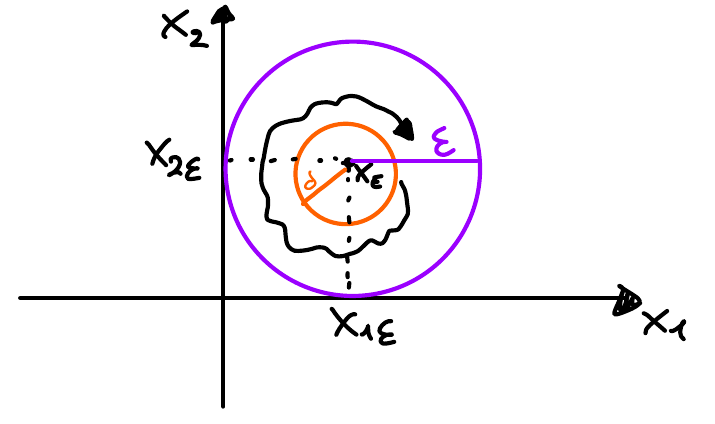
\includegraphics[scale=0.3]{Images/Equilibrio_stabile.png}
\end{center}

\subsubsection*{Rappresentazione grafica di un sistema in equilibrio attrattivo}
\begin{center}
    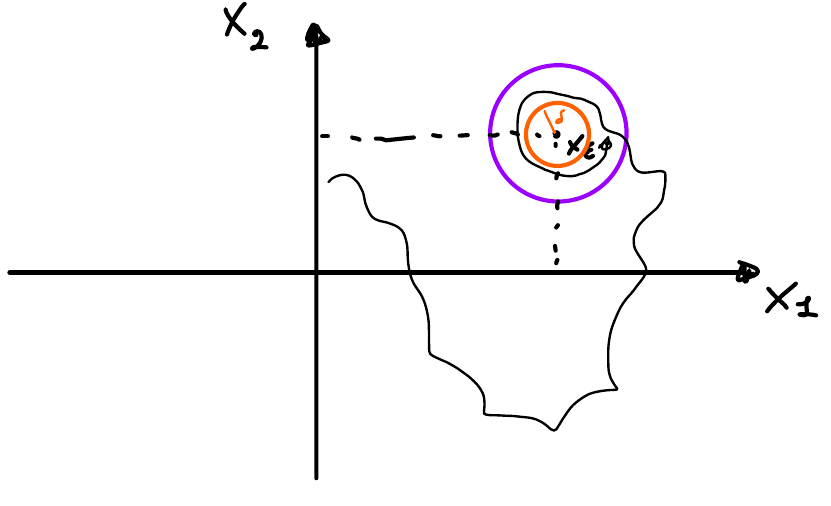
\includegraphics[scale=0.3]{Images/Equilibrio_attrattivo.png}
\end{center}

\subsubsection{Osservazioni}
Le definizioni date sottintendono la parola locale, ovvero che la proprietà vale in un intorno dello stato di equilibrio $x_e$.
\vspace*{0.2cm}\\
\textbf{Stabilità globale:} le proprietà di stabilità e asintotica stabilità sono globali se valgono per ogni $x \in \mathbb{R}^n$, invece che valere solo per $x_0$ tale che $|| x(0)-x_e || \leq \delta $.
\vspace*{0.2cm}\\
\textbf{Stabilità di una traiettoria:} le definizioni di stabilità si possono generalizzare a una traiettoria $\overline{x}(t), t \geq 0$.
\begin{center}
    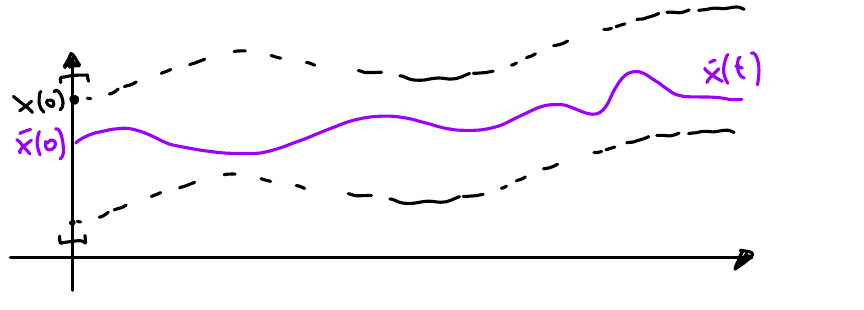
\includegraphics[scale=0.3]{Images/Stabilita_traiettoria.png}
\end{center}

\subsection{Stabilità interna di sistemi LTI}
Nei sistemi lineari $x=0$ è sempre un equilibrio.\\
Per sistemi lineari si può dimostrare che tutti gli equilibri e tutte le traiettorie hanno le stesse proprietà di stabilità, tutte uguali a $x=0$. Per questo motivo si parla di \textbf{stabilità del sistema}.
\subsubsection*{Dimostrazione}
\begin{equation}
    \begin{rcases}
        \dot x(t) = Ax(t) + Bu(t)\\
        u(t) = u_e \ \ \forall t \geq 0
    \end{rcases}
    \Longrightarrow Ax_e + Bu_e = 0
\end{equation}
Sia $\tilde{x}(t) := x(t) - x_e$, allora
\begin{align*}
    \dot{\tilde{x}}(t) &= \dot x(t) - \underbrace{\frac{d}{dt}x_e}_{0}\\
    &=Ax(t)+Bu_e\\
    &=A(\tilde{x}(t)+x_e)+Bu_e\\
    &=A \tilde{x}(t) + \underbrace{Ax_e+Bu_e}_{0}
\end{align*}
quindi
\begin{equation}
    \dot{\tilde{x}}(t) = A \tilde{x}(t)
\end{equation}
Concludiamo che
\begin{equation}
    \tilde{x}=0 \Longleftrightarrow x = x_e
\end{equation}
cioè per studiare l'equilibrio di un sistema nel generico punto $x_e$ posso studiare l'equilibrio del sistema nell'origine.




\subsubsection*{Teorema} \label{Teorema parte reale negativa}
Un sistema LTI è \textbf{asintoticamente stabile} \underline{se e solo se} tutti gli autovalori hanno parte reale strettamente negativa.
\vspace*{0.1cm}\\
\textbf{N.B.} Se gli autovalori hanno parte reale strettamente negativa i modi del sistema tendono a 0 (\ref{Modi naturali: autovalori reali semplici}).

\subsubsection*{Teorema}
Un sistema LTI è stabile se e solo se tutti gli autovalori hanno parte reale minore o uguale a zero e tutti gli autovalori a parte reale nulla hanno molteplicità geometrica uguale alla molteplicità algebrica (i mini blocchi di Jordan associati hanno dimensione uno).

\subsubsection*{Osservazione}
Si ha instabilità se almeno un autovalore ha parte reale positiva o se almeno un autovalore con parte reale nulla ha molteplicità algebrica maggiore della molteplicità geometrica.


\subsubsection*{Osservazione}
La stabilità asintotica di sistemi LTI è sempre globale
\begin{align*}
    x(0) &= x_0 \Longrightarrow x(t) \ \ t \geq 0 \\
    x(0) &= \alpha x_0 \Longrightarrow \alpha x(t) \ \ t \geq 0
\end{align*}


\subsubsection*{Proprietà}
Se un sistema LTI è globalmente asintoticamente stabile, $x=0$ è l'unico equilibrio.\\
\textbf{Nota:} anche per sistemi \underline{non lineari} se $x_e$ è GAS (Globalmente Asintoticamente Stabile) allora è l'unico equilibrio.
\vspace*{0.1cm}\\
Questo perché



\subsubsection{Esempio stabilità del sistema carrello}
\begin{align*}
    \dot x_1(t) &= x_2(t) \\
    \dot x_2(t) &= - \frac{k(t)}{M}x_1(t) + \frac{1}{M} u(t) \\
    y(t) &= x_1(t)
\end{align*}
\begin{align*}
    \begin{bmatrix}
        \dot x_1(t)\\
        \dot x_2(t)
    \end{bmatrix} &=
    \begin{bmatrix}
        0 & 1\\
        - \frac{k}{M} & 0
    \end{bmatrix}
    \begin{bmatrix}
        x_1(t)\\
        x_2(t)
    \end{bmatrix}
    +
    \begin{bmatrix}
        0\\
        \frac{1}{M}
    \end{bmatrix} u(t)
    \\
    y(t) &= \begin{bmatrix}
        1 & 0
    \end{bmatrix}
    \begin{bmatrix}
        x_1(t)\\
        x_2(t)
    \end{bmatrix} + 0 u(t)
\end{align*}
Consideriamo $k$ costante, quindi sistema LTI.\\
Gli autovalori della matrice $A$ sono $\lambda_1 = j \sqrt{\dfrac{k}{M}}, \lambda_2 = -j \sqrt{\dfrac{k}{M}}$ immaginari puri, quindi sistema semplicemente (marginalmente) stabile.
\vspace*{0.2cm}\\
Se applichiamo $u=-h x_2$ gli autovalori diventano $\lambda_1 = - \frac{h}{2M} + \sqrt{\dfrac{h^2}{4M^2}-\dfrac{k}{M}}$ e $\lambda_2 = \dfrac{h}{2M} - \sqrt{\dfrac{h^2}{4M^2}-\dfrac{k}{M}}$.\\
\begin{itemize}
    \item Se $h^2 \geq 4Mk$ gli autovalori sono 2 reali negativi, quindi il sistema è asintoticamente stabile;
    \item Se $h^2 < 4Mk$ gli autovalori sono 2 complessi coniugati con parte reale negativa, quindi il sistema è asintoticamente stabile;
    \item Se $h^2 = 4Mk$, $\lambda_1 = \lambda_2 = -\frac{h}{2M}$, con molteplicità algebrica pari a 2. Si può dimostrare che la molteplicità geometrica è pari a 1, quindi il blocco di Jordan sarà $2 \times 2$ (guardare \ref{proprietà della matrice esponenziale})
    \begin{align*}
        J &= TAT^{-1} = 
        \begin{bmatrix}
            - \frac{h}{2M} & 1\\
            0 & - \frac{h}{2M}
        \end{bmatrix}
        &
        e^{Jt} &= e^{- \frac{h}{2M}t}
        \begin{bmatrix}
            1 & t\\
            0 & 1
        \end{bmatrix}
    \end{align*}
    Gli autovalori sono a parte reale negativa, quindi il sistema è asintoticamente stabile;
    \item Se $h=k=0 \Longrightarrow \lambda_1=\lambda_2=0$, quindi il sistema è instabile.
\end{itemize}





\subsection{Retroazione dello stato}
Prendiamo un sistema lineare tempo invariante
\begin{align*}
    \dot x(t) &= Ax(t) + Bu(t)\\
    y(t) &= Cx(t) + Du(t) 
\end{align*}
Supponendo di misurare l'intero stato, ovvero se $x(t)=y(t)$, allora possiamo progettare
\begin{equation}
    u(t) = Kx(t) + v(t)
\end{equation}
con $K \in \mathbb{R}^{m \times n}$ una matrice di guadagni e $v(t)$ un ulteriore ingresso per il sistema retroazionato
\begin{equation}
    \dot x(t) = (A+BK)x(t)+Bv(t)
\end{equation}
Se vogliamo il sistema in anello chiuso asintoticamente stabile allora dobbiamo progettare $K$ tale che $(A + BK)$ abbia autovalori tutti a parte reale negativa.\\
\textbf{Nota:} la possibilità di scegliere gli autovalori di $(A + BK)$ (e.g., per renderli tutti a parte reale negativa) dipende dalla coppia $(A, B)$ ed è legata alla proprietà di \textbf{raggiungibilità}.
\vspace*{0.1cm}\\
Se non è possibile misurare l'intero stato, ovvero se $y(t) \neq x(t)$, esistono tecniche per ricostruire lo stato a partire dalle misure mediante sistemi ausiliari chiamati \textbf{osservatori}.\\
Se sia possibile o meno ricostruire lo stato dipende dalla coppia $(A, C)$ ed è legato alla proprietà di \textbf{osservabilità}.




\subsection{Linearizzazione di sistemi in non lineari (tempo invarianti)}
Prendiamo un  sistema non lineare tempo invariante
\begin{align*}
    \dot x(t) &= f (x(t), u(t))\\
    y(t) &= h(x(t), u(t))
\end{align*}
Sia $(x_e,u_e)$ una coppia di equilibrio, $f(x_e,u_e)=0$, consideriamo una traiettoria a partire da uno stato stato iniziale $x(0)=x_e+ \tilde{x}_0$ 
\begin{align*}
    x(t) &= x_e + \tilde{x}(t)\\
    u(t) &= u_e + \tilde{u}(t)
\end{align*}
con $y(t) = h(x_e , u_e ) + \tilde{y}(t) = y_e + \tilde{y}(t)$.\\
Essendo una traiettoria vale
\begin{align*}
    \frac{d}{dt}(x_e + \tilde{x}(t)) &= f (x_e + \tilde{x}(t), u_e + \tilde{u}(t))\\
    y_e + \tilde{y}(t) &= h(x_e+\tilde{x}(t), u_e+ \tilde{u}(t))
\end{align*}
Sviluppando in serie di Taylor (con $f$ e $h$ sufficientemente regolari) in $(xe , ue )$ \footnote[1]{i termini del tipo $\frac{\partial}{\partial x}f(x,u)$ vengono chiamati \textit{Jacobiani}}
\begin{align*}
    \frac{d}{dt}(x_e + \tilde{x}(t)) &= \underbrace{f(x_e,u_e)}_{0} + \underbrace{\frac{\partial}{\partial x}f(x,u)\bigg|_{\substack{\text{$x=x_e$} \\ \text{$u=u_e$}}}}_{A_e} \tilde{x}(t) + \underbrace{\frac{\partial}{\partial u}f(x,u)\bigg|_{\substack{\text{$x=x_e$} \\ \text{$u=u_e$}}}}_{B_e} \tilde{u(t)} + \T{term. ord. sup.}\\
    y_e+\tilde{y}(t) &= h(x_e,u_e) + \frac{\partial}{\partial x}h(x,u) \bigg|_{\substack{\text{$x=x_e$} \\ \text{$u=u_e$}}} \tilde{x}(t) + \frac{\partial}{\partial u}h(x,u) \bigg|_{\substack{\text{$x=x_e$} \\ \text{$u=u_e$}}} \tilde{u}(t) + \T{term. ord. sup.}
\end{align*} 
quindi
\begin{align*}
    \tilde{\dot x}(t) &= A_e \tilde{x}(t) + B_e \tilde{u}(t) + \T{term. ord. sup.} \tag*{$\tilde{x}(0) = \tilde{x}_0$}\\
    \tilde{y}(t) &= C_e \tilde{x}(t) + D_e\tilde{u}(t) + \T{term. ord. sup.}
\end{align*}
Se consideriamo i termini di ordine superiore come un resto $\mathcal{R}(x,u)$ si osserva che
\begin{equation}
    \lim_{||(x,u)||\rightarrow 0} \frac{||\mathcal{R}(\tilde{x},\tilde{u})||}{||(\tilde{x},\tilde{u})||} = 0
\end{equation}
di fatto è come se si avesse $\lim\limits_{x \rightarrow 0}\dfrac{x^2}{x}$.\\
Quindi le due equazioni di prima si possono approssimare
\begin{align*}
    \tilde{\dot x}(t) &\approx A_e \tilde{x}(t) + B_e \tilde{u}(t)\\
    \tilde{y}(t) &\approx C_e \tilde{x}(t) + D_e\tilde{u}(t) 
\end{align*}
Il sistema linearizzato è
\begin{align*}
    \Delta \dot x(t) &= A \Delta x(t) + B \Delta u(t)\\
    \Delta y(t) &= C \Delta x(t) + D \Delta u(t)
\end{align*} 
Le traiettorie del sistema non lineare soddisfano
\begin{align*}
    x(t) &= x_e + \tilde{x}(t) \approx x_e + \Delta x(t)\\
    u(t) &= u_e + \tilde{u}(t) \approx u_e + \Delta u(t)\\
    y(t) &= y_e + \Delta y(t) \approx y_e + \Delta y(t) 
\end{align*}
per variazioni sufficientemente piccole.
\vspace*{0.1cm}\\
\textbf{Nota:} $(\Delta x(t),\Delta u(t)), t \geq 0$ traiettoria del sistema linearizzato.



\subsubsection{Esempio pendolo}
\begin{align*}
    \dot x_1(t) &= x_2(t) = f_1(x(t),u(t))\\
    \dot x_2(t) &= - \frac{g}{l} \sin(x_1(t)) - \frac{b}{M \ell^2}x_2(t) + \frac{1}{M \ell^2} u(t) = f_2(x(t),u(t))
\end{align*}
$(x_e,u_e)$ coppia di equilibrio
\begin{equation}
    f(x_e,u_e)=0 \Rightarrow 
    \begin{cases}
        x_{2e}=0\\
        - \dfrac{g}{\ell} \sin(x_{1e}) - \dfrac{b}{M \ell^2}x_{2e} + \dfrac{1}{M \ell^2}u_e
    \end{cases}
\end{equation}
Prendiamo come equilibrio $x_e = \begin{bmatrix} x_{1e}\\0 \end{bmatrix}$, allora
\begin{align*}
    &- \dfrac{g}{\ell} \sin(x_{1e}) - \dfrac{b}{M \ell^2} \cdot 0 + \dfrac{1}{M \ell^2}u_e = 0\\
    \Longrightarrow & u_e = gM\ell \sin(X_{1e})
\end{align*}
Eseguiamo la linearizzazione intorno a $(x_e,u_e)$
\begin{equation}
    \Delta \dot x(t) = A_e \Delta x(t) + B_e \Delta u(t)
\end{equation}
%calcolo matrice A_e
\begin{align*}
    \underbrace{A_e}_{\frac{\partial f(x,u)}{\partial x}\big|_{\substack{\text{$x=x_e$} \\ \text{$u=u_e$}}}} &=
    \begin{bmatrix}
        \dfrac{\partial f_1(x,u)}{\partial x_1} & \dfrac{\partial f_1(x,u)}{\partial x_2}\\
        \dfrac{\partial f_2(x,u)}{\partial x_1} & \dfrac{\partial f_2(x,u)}{\partial x_2}
    \end{bmatrix}_{\substack{\text{$x=x_e$} \\ \text{$u=u_e$}}}\\ &=
    \begin{bmatrix}
        0 & 1\\
        -\dfrac{g}{\ell}\cos(x_1) & -\dfrac{b}{M \ell^2}
    \end{bmatrix}_{\substack{\text{$x=x_e$} \\ \text{$u=u_e$}}} \\ &=
    \begin{bmatrix}
        0 & 1\\
        -\dfrac{g}{\ell}\cos(x_{1e}) & -\dfrac{b}{M \ell^2}
    \end{bmatrix}
\end{align*}
%calcolo matrice B_e
\begin{align*}
    \underbrace{B_e}_{\frac{\partial f(x,u)}{\partial u}\big|_{\substack{\text{$x=x_e$} \\ \text{$u=u_e$}}}} &=
    \begin{bmatrix}
        \dfrac{\partial f_1(x,u)}{\partial u}\\
        \dfrac{\partial f_2(x,u)}{\partial u} 
    \end{bmatrix}_{\substack{\text{$x=x_e$} \\ \text{$u=u_e$}}}\\ &=
    \begin{bmatrix}
        0\\
        \dfrac{1}{M \ell^2}
    \end{bmatrix}_{\substack{\text{$x=x_e$} \\ \text{$u=u_e$}}}\\ &=
    \begin{bmatrix}
        0\\
        \dfrac{1}{M \ell^2}
    \end{bmatrix}
\end{align*}
\begin{itemize}
    \item se $x_e = \begin{bmatrix} 0\\0 \end{bmatrix}$ e $u_e = 0$
    \begin{align*}
        A_e &= 
        \begin{bmatrix}
            0 & 1\\
            -\dfrac{g}{\ell} & -\dfrac{b}{M \ell^2}
        \end{bmatrix} 
        &
        B_e &=
        \begin{bmatrix}
            0\\
            \dfrac{1}{M \ell^2}
        \end{bmatrix}
    \end{align*}
    \item se $x_e=\begin{bmatrix} \pi\\0 \end{bmatrix}$ e $u_e=0$
    \begin{align*}
        A_e &= 
        \begin{bmatrix}
            0 & 1\\
            \dfrac{g}{\ell} & -\dfrac{b}{M \ell^2}
        \end{bmatrix} 
        &
        B_e &=
        \begin{bmatrix}
            0\\
            \dfrac{1}{M \ell^2}
        \end{bmatrix}
    \end{align*}
    \item se $x_e=\begin{bmatrix} \pi/2 \\0 \end{bmatrix}$ e $u_e=MG\ell$
    \begin{align*}
        A_e &= 
        \begin{bmatrix}
            0 & 1\\
            0 & -\dfrac{b}{M \ell^2}
        \end{bmatrix} 
        &
        B_e &=
        \begin{bmatrix}
            0\\
            \dfrac{1}{M \ell^2}
        \end{bmatrix}
    \end{align*}
\end{itemize}



\subsubsection{Stabilità di 3 sistemi lineari (linearizzzione intorno a 3 diversi equilibri)}
\begin{enumerate}
    \item 
    \begin{align*}
        A_e &= \begin{bmatrix} 0&1\\-\dfrac{g}{\ell}&-\dfrac{b}{M \ell^2} \end{bmatrix} & p(\lambda) &= \lambda \left( \lambda + \frac{b} +{M\ell^2} \right) + \frac{g}{\ell}\\
        & & &=\lambda^2 + \frac{b}{M\ell^2}\lambda + \frac{g}{\ell}
    \end{align*}
    \begin{equation}
        \lambda_{1/2} = - \frac{b}{2M \ell^2} \pm \sqrt{\left(\frac{b}{2M\ell^2}\right) - \frac{g}{\ell}}
    \end{equation}
    Abbiamo 2 autovalori a parte reale negativa, quindi il sistema linearizzato è \textit{asintoticamente stabile (globalmente)}.

    \item 
    \begin{align*}
        A_e &= \begin{bmatrix} 0&1\\\dfrac{g}{\ell}&-\dfrac{b}{M \ell^2} \end{bmatrix} & p(\lambda) &= \lambda \left( \lambda + \frac{b} {M\ell^2} \right) - \frac{g}{\ell}\\
        & & &=\lambda^2 + \frac{b}{M\ell^2}\lambda - \frac{g}{\ell}
    \end{align*}
    \begin{equation}
        \lambda_{1/2} = - \frac{b}{2M \ell^2} \pm \sqrt{\underbrace{\left(\frac{b}{2M\ell^2}\right) + \frac{g}{\ell}}_{>0}} \Longrightarrow
        \begin{cases}
            \lambda_{1} = - \dfrac{b}{2M \ell^2} - \sqrt{\left(\dfrac{b}{2M\ell^2}\right) + \dfrac{g}{\ell}} <0\\
            \\
            \lambda_{2} = - \dfrac{b}{2M \ell^2} + \sqrt{\left(\dfrac{b}{2M\ell^2}\right) + \dfrac{g}{\ell}} >0
        \end{cases}
    \end{equation}
    Dato che abbiamo un autovalore a parte reale positiva il sistema è \textit{instabile}.

    \item 
    Se poniamo $x_e = \begin{bmatrix} \pi/2\\ 0 \end{bmatrix}$ e $M_e = Mg\ell$
    \begin{align*}
        A_e &= \begin{bmatrix} 0&1\\ 0&-\dfrac{b}{M \ell^2} \end{bmatrix} & p(\lambda) &= \lambda \left( \lambda + \frac{b} {M\ell^2} \right)
    \end{align*}
    \begin{align*}
        \lambda_1 &= 0 & \lambda_2&=-\frac{b}{M\ell^2}
    \end{align*}
    Il sistema linearizzato è \textit{stabile}, ma non asintoticamente, cioè marginalmente stabile (ricordando \ref{Teorema parte reale negativa})
\end{enumerate}



\subsection{Stabilità e linearizzazione}
\subsubsection*{Teorema}
Dato un sistema non lineare tempo invariante, $\dot x(t)=f(x(t),u(t))$, sia $x_e,u_e$ una coppia di equilibrio. Se il sistema linearizzato intorno a $(x_e,u_e)$ è asintoticamente stabile, allora l'equilibrio $x_e$, relativo all'ingresso $u_e$, è (localmente) asintoticamente stabile.

\subsubsection*{Teorema}
Dato un sistema non lineare tempo invariante, $\dot x(t)=f(x(t),u(t))$, sia $x_e,u_e$ una coppia di equilibrio. Se il sistema linearizzato intorno a $(x_e,u_e)$ ha almeno un autovalore a parte reale positiva, allora l'equilibrio $x_e$, relativo all'ingresso $u_e$, è instabile.


\subsubsection{Controllo nonlineare mediante linearizzazione}
Consideriamo il sistema non lineare
\begin{equation}
    \dot x(t) = f(x(t),u(t))
\end{equation}
Linearizzazione intorno all'equilibrio $(x_e,u_e)$
\begin{equation}
    \Delta \dot x(t) = A_e \Delta x(t) + B_e \Delta u(t)
\end{equation}
Proviamo a portare $\Delta x(t)$ a 0, ovvero $x(t)$ a $x_e$ "in modo approssimato". Usando la retroazione dello stato $\Delta u(t) = K \Delta x(t) + \Delta v(t)$ otteniamo il seguente sistema in anello chiuso
\begin{equation}
    \Delta \dot x(t) = (A_e + B_e K)\Delta x(t) + B_e \Delta v(t)
\end{equation}
Così sono in grado di progettare la matrice $K$ in modo che $A_e + B_e K$ sia asintoticamente stabile. Grazie ai teoremi sulla linearizzazione, $x_e$ risulta un equilibrio (localmente) asintoticamente stabile per il sistema non lineare in anello chiuso (detto \textit{retroazionato}).
\vspace*{0.1cm}\\
Visto che $\Delta x(t) \approx x(t) - x_e$
\begin{equation}
    u(t) = u_e + K(x(t) - x_e) + \tilde{v}(t) \approx u_e + K \Delta x(t) + \tilde{v}(t)
\end{equation}
Perciò la legge di controllo finale sarà
\begin{equation}
    u(t) = u_e + K(x(t)-x_e) + \tilde{v}(t)
\end{equation}
\begin{center}
    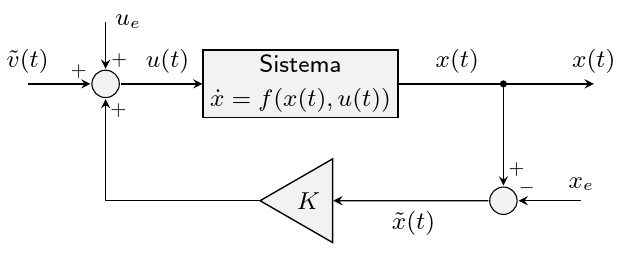
\includegraphics[scale=0.4]{Images/Controllo_retroazionato.png}
\end{center}
 




\section{Trasformata di Laplace}
\subsection{Definizione}
Data una funzione complessa $f$ di variabile reale $t$, $f: \mathbb{R} \rightarrow \mathbb{C}$ (anche se per noi tipicamente saranno funzioni $f: \mathbb{R} \rightarrow \mathbb{R}$), sia $s = \sigma + j \omega$ una variabile complessa ($\sigma$ parte reale, $\omega$ parte immaginaria); definiamo la \textit{Trasformata di Laplace} di $f(t)$
\begin{equation}
    F(s) = \int_{0^-}^{+ \infty} f(t) e^{-st} \ dt
\end{equation}
se esiste per qualche $s$, ovvero se l'integrale converge.\\
Includiamo nell'integrale $0^{-}$ per tener conto di eventuali impulsi cone la \textit{delta di Dirac}.
\vspace*{0.2cm}\\
\textbf{Notazione:} indichiamo la trasformata di Laplace con $\mathcal{L}$ tale che
\begin{equation}
    f(t) \overset{\mathcal{L}}{\xrightarrow{\hspace*{0.8cm}}} F(s)
\end{equation}
con $F:\mathbb{C} \rightarrow \mathbb{C}$; indichiamo l'applicazione della trasformata con $F(s) = \mathcal{L}[f(t)]$.


\subsection{Osservazioni}
\subsubsection{Ascissa di convergenza}
Sia $\overline{\sigma}>- \infty$ estremo inferiore di $s=\sigma + j \omega$ per cui l'integrale converge. Allora la trasformata di Laplace esiste nel semipiano $\operatorname{Re} (s)>\overline{\sigma}$. $\overline{\sigma}$ viene chiamata \textit{ascissa di convergenza}.\\
La trasformata di Laplace risulta essere una \textit{funzione analitica} e, grazie alle particolari proprietà delle funzioni analitiche, la sua definizione può essere estesa anche in punti $s$ tali che $ \operatorname{Re}(s)\leq \overline{\sigma}$, indipendentemente dal fatto che l'integrale non converga.
\vspace*{0.2cm}\\
Dato che 
\begin{equation}
    e^{-st} = e^{- \sigma t}e^{-j \omega t}
\end{equation}
possiamo dire che $e^{-\sigma t}$ ci aiuta a ottenere un integrale che converge.
\begin{center}
    \begin{tikzpicture}
            \begin{axis}[
                xmin=0,xmax=5,
                ymin=0,ymax=1,
                ticks=none, %elimina i valori numerici
                axis x line=middle,
                axis y line=middle,
                xlabel={$x$},
                ylabel={$y$},
                ]
                \addplot[domain=0.05:4.5, samples=100]{exp(-x)}node [pos=0.1,anchor=south west]{$e^{-\sigma t}$};
            \end{axis}
        \end{tikzpicture}
    \end{center}
\subsubsection{Trasformate razionali}
Di particolare importanza sono le \textit{trasformate razionali}, cioè quelle in cui
\begin{equation}
    F(s) = \frac{N(s)}{D(s)}
\end{equation}
con $N(s)$ e $D(s)$ polinomi primi tra loro. Le radici di $N(s)=0$ si dicono \textbf{zeri} e quelle di $D(s)=0$ si dicono \textbf{poli}: nell'insieme, poli e zeri si dicono \textit{singolarità}.
\vspace*{0.1cm}\\
Se $f$ è reale allora i coefficienti dei polinomi $N(s)$ e $D(s)$ sono reali.

\subsubsection*{Esempio}
\begin{equation}
    F(s) = \frac{s^2+2s}{(s+1)(s+3)} = \frac{s(s+2)}{(s+1)(s+3)}
\end{equation}
allora
\begin{itemize}
    \item zeri di $F(s)$: $0$ e $-2$
    \item poli di $F(s)$: $-1$ e $-3$
\end{itemize}


\subsection{Formula di antitrasformazione}
La funzione trasformanda può essere ricavata dalla sua trasformata
mediante la \textit{formula di antitrasformazione}
\begin{equation}
    f(t) = \frac{1}{2 \pi j} \int _{\sigma-j \infty}^{\sigma+j \infty} F(s) e^{st} \ ds
\end{equation}
\textbf{Notazione:} indichiamo l'antitrasformata di Laplace con $\mathcal{L}^{-1}$ tale che
\begin{equation}
    F(s) \overset{\mathcal{L}^{-1}}{\xrightarrow{\hspace*{0.8cm}}} f(t) \tag*{$\sigma > \overline{\sigma}$}
\end{equation}
indichiamo la formula di antitrasformazione con $f(t) = \mathcal{L}^{-1}[F(s)]$.
\vspace*{0.2cm}\\
La $f(t)$ è fornita per $t\geq 0$, perché solo nei punti di continuità in cui la $f$ è maggiore di zero essa contribuisce a determinare $F$. L'antitrasformata fornisce $f(t)=0$ per $t<0$, per questo la corrispondenza tra $f(t)$ e $F(s)$ è \textbf{biunivoca}.


\subsubsection{Perché si utilizza la trsformata di Laplace}
\begin{center}
    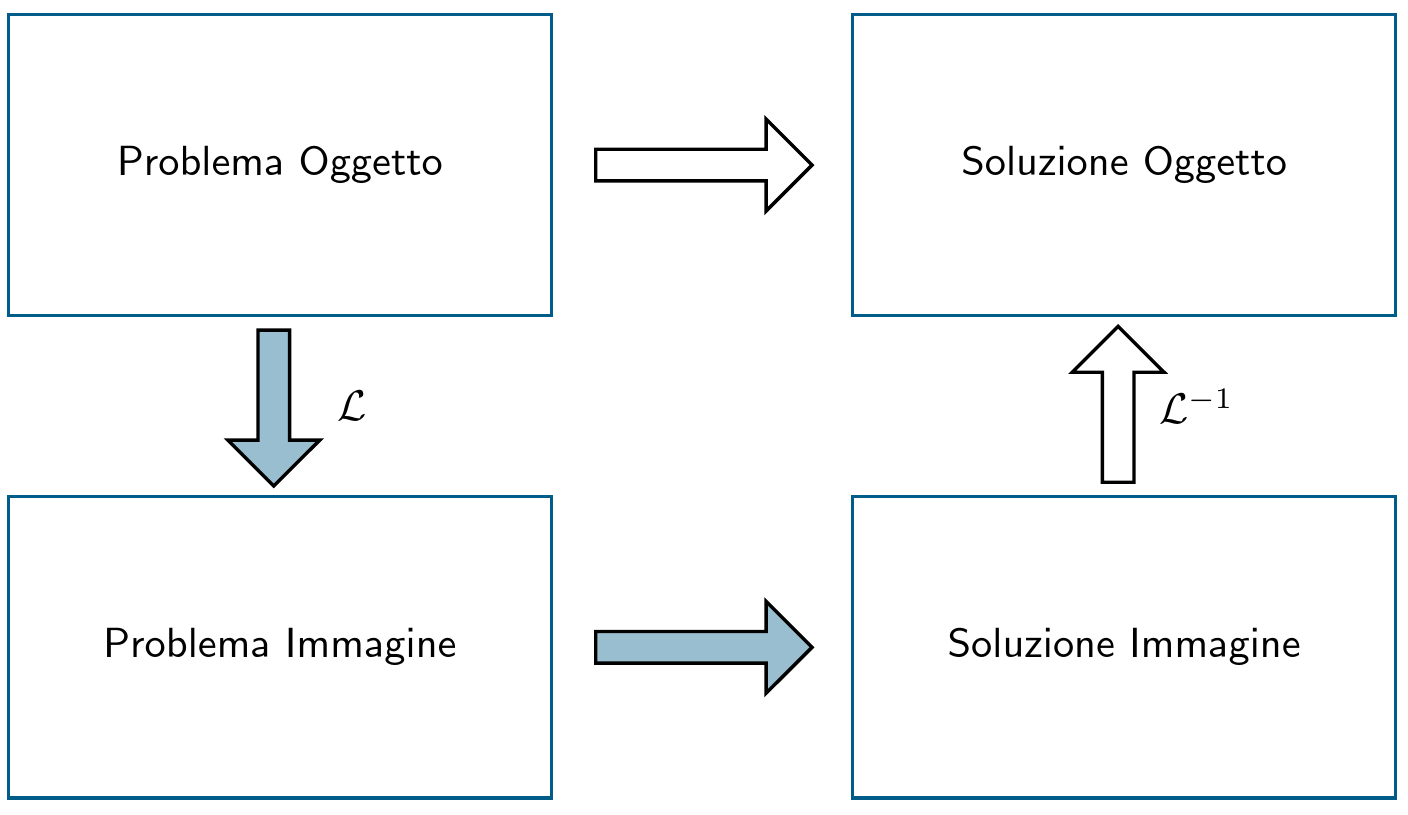
\includegraphics[scale=0.18]{Images/Motivo_Laplace.png}
\end{center}
Se, provando a risolvere il problema oggetto, risulta difficile arrivare alla soluzione oggetto (magari perché i calcoli sono molto complessi o risulta poco conveniente in termini di risorse), allora si trasforma il problema oggetto in problema immagine con la trasformata di Laplace se risulta poi conveniente (o semplice) arrivare alla soluzione immagine, per poi antitrasformarla per ottenere la soluzione oggetto che si stava cercando.


\subsection{Proprietà della trasformata di Laplace}
\subsubsection{Linearità}
Dati $f(t)$ e $g(t)$ tali per cui esistono le trasformate $F(s)$ e $G(s)$, allora $\forall \alpha \in \mathbb{C}, \forall \beta \in \mathbb{C}$ risulta
\begin{equation}
    \mathcal{L}[\alpha f(t) + \beta g(t)] = \alpha \mathcal{L}[f(t)] + \beta \mathcal{L}[g(t)] = \alpha F(s) + \beta G(s)
\end{equation}

\subsubsection*{Dimostrazione}
\begin{align*}
    \mathcal{L}[\alpha f(t) + \beta g(t)] &= \int_{0^{-}}^{+\infty}\left(\alpha f(t) + \beta g(t)\right) e^{-st} \ dt\\
    &= \alpha \underbrace{\int_{0^{-}}^{+\infty} f(t)e^{-st} \ dt}_{F(s)} + \beta \underbrace{\int_{0^{-}}^{+\infty} g(t)e^{-st} \ dt}_{G(s)}\\
    &= \alpha F(s) + \beta G(s)
\end{align*}

\subsubsection{Traslazione temporale}
\begin{equation}
    \mathcal{L}[f(t-\tau)] = e^{-\tau s}F(s) \tag*{$\forall \tau >0$}
\end{equation}
$\tau$ deve essere maggiore di 0, altrimenti la $f(t)$ sarebbe diversa da 0 per un tempo negativo.

\subsubsection*{Dimostrazione}
\begin{align*}
    \mathcal{L}[f(t-\tau)] &= \int_{0^-}^{+ \infty} f(t - \tau)e^{-st} \ dt\\
    &\underset{\rho = t-\tau}{=} \int_{-\tau^-}^{+ \infty} f(\rho)e^{-s(\rho+t)} \ d\rho\\
\end{align*}
siccome la $f(t)$ è nulla per $t<0$ posso riscrivere gli estremi di integrazione
\begin{align*}
    \int_{0^-}^{+ \infty} f(\rho)e^{-s(\rho+t)} \ d\rho
    &= \underbrace{\int_{0^-}^{+ \infty} f(\rho)e^{\rho} \ d\rho}_{F(s)} \cdot e^{-s\tau} \\
    &= F(s) e^{-s\tau}
\end{align*}
come volevasi dimostrare
\begin{equation}
    \mathcal{L}[f(t-\tau)] = e^{-\tau s}F(s)
\end{equation}

\subsubsection{Traslazione nel dominio della variabile complessa}\label{Traslazione nel dominio della variabile complessa}
\begin{equation}
    \mathcal{L}[e^{\alpha t }f(t)] = F(s - 
    \alpha)
\end{equation}

\subsubsection*{Dimostrazione}
\begin{align*}
    \mathcal{L}[e^{\alpha t }f(t)] &= \int_{0^-}^{+ \infty} f(t)e^{\alpha t} \cdot e^{-st} \ dt \\
    &= \int_{0^-}^{+ \infty} f(t)e^{-(s-\alpha)t} \ dt\\
    &= F(s-\alpha)
\end{align*}

\subsubsection{Derivazione nel dominio del tempo}\label{Derivazione nel dominio del tempo}
\begin{equation}
    \mathcal{L}\left[\frac{d}{dt}f(t)\right] = sF(s) - f(0)
\end{equation}
Calcoliamo la trasformata della derivata seconda
\begin{align*}
    \mathcal{L}\left[\frac{d^2}{dt^2}f(t)\right] &=
    \mathcal{L}\left[\frac{d}{dt}\underbrace{\left[\frac{d}{dt}f(t)\right]}_{g(t)}\right]\\
    &=sG(s) - g(0)\\
    &=sG(s) - f'(0)\\
    &=s(sF(s)-f(0)) - f'(0)\\
    &= s^2 F(s) - sf(0) - f'(0)
\end{align*}
Quindi possiamo definire la \textit{derivata n-sima nel tempo}
\begin{equation}
    \mathcal{L}\left[\frac{d^n}{dt^n}f(t)\right] = s^nF(s) = \sum_{i=1}^n s^{n-i} \frac{d^{i-1}}{dt^{i-1}}f(t)|_{t=0}
\end{equation}
La proprietà ci dice che, se la funzione e le sue derivate si annullano in $t=0$, derivare nel dominio del tempo equivale a moltiplicare per $s$ nel dominio della variabile complessa; infatti $s$ viene chiamato \textit{operatore di derivazione}.


\subsubsection{Derivazione nel dominio della variabile complessa}\label{Derivazione nel dominio della variabile complessa}
Supponiamo $F(s)$ derivabile per tutti gli $s$; allora risulta
\begin{equation}
    \mathcal{L}[t f(t)] = - \frac{dF(s)}{ds}
\end{equation}
la quale è estendibile al caso della trasformata $t^n \cdot f(t)$.

\subsubsection*{Dimostrazione}
Considerando che $te^{-st} = -\dfrac{d}{ds}e^{-st}$
\begin{align*}
    \mathcal{L}[t f(t)] &= \int_{0^+}^{+\infty} t f(t)e^{-st} \ dt\\
    &=\int_{0^+}^{+\infty} f(t) \underbrace{te^{-st}}_{-\frac{d}{ds}e^{-st}} \ dt\\
    &=\int_{0^+}^{+\infty} f(t) \left(-\frac{d}{ds}e^{-st}\right) \ dt\\
    &=-\frac{d}{ds} \underbrace{\int_{0^+}^{+\infty} f(t) e^{-st} \ dt}_{F(s)}\\
    &= - \frac{dF(s)}{ds}
\end{align*}


\subsubsection{Integrazione nel tempo}
Supponiamo che la funzione $f(t)$ sia integrabile tra 0 e $+ \infty$. Allora
\begin{equation}
    \mathcal{L} \left[\int_0^tf(\tau) \ d\tau\right] = \frac{1}{s} F(s)
\end{equation}
La proprietà ci dice che integrare nel dominio del tempo equivale a dividere per $s$ nel dominio della variabile complessa; infatti $\dfrac{1}{s}$ viene chiamato \textit{operatore di integrazione}.


\subsubsection{Convoluzione nel tempo}
Date due funzioni $f_1$ e $f_2$, il loro \textit{prodotto di convoluzione} è
\begin{equation}
    f_1(t) \ast f_2(t) = \int_{-\infty}^{+\infty} f_1(t -\tau)f_2(t) \ d\tau = \int_{-\infty}^{+\infty} f_1(\eta)f_2(\eta) \ d\eta = f_2(t-\eta) \ast f_1(t)
\end{equation}
e si trova
\begin{equation}
    \mathcal{L}[f_1(t) \ast f_2(t)] = F_1(s) \cdot F_2(s)
\end{equation}

\subsubsection{Teorema del valore iniziale}
Se una funzione reale $f(t)$ ha trasformata razionale $F(s)$ con grado del denominatore maggiore del grado del numeratore, allora
\begin{equation}
    f(0) = \lim_{s\rightarrow \infty} s F(s)
\end{equation}
Se $f$ è una funzione discontinua di prima specie in $t=0$, $f(0)$ si interpreta come $f(0^+)$. L'equazione vale se $f(0)$ o $f(0^+)$ esistono.


\subsubsection{Teorema del valore finale}
Se una funzione reale $f(t)$ ha trasformata razionale $F(s)$ con grado del denominatore maggiore del grado del numeratore e poli nulli o con parte reale negativa, allora
\begin{equation}
    \lim_{t \rightarrow + \infty} f(t) = \lim_{s\rightarrow 0} s F(s)
\end{equation}
L'equazione vale se esiste $\lim\limits_{t \rightarrow + \infty}f(t)$ esiste.


\subsection{Trasformata di segnali elementari}
Definiamo il \textit{delta di Dirac} $\delta(t)$ tale che
\begin{equation}
    \int_{0^-}^{0^+} \delta(t) \ dt = 1
\end{equation}
\begin{center}
    \renewcommand{\arraystretch}{5}
    \begin{tabular}{c c}
        $\mathcal{L}[\delta(t)]=1$ & 
        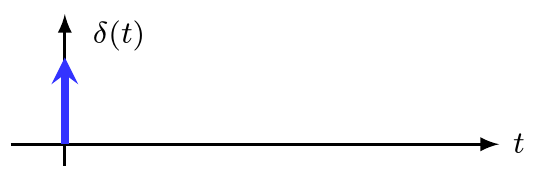
\includegraphics[width=0.25\linewidth, valign=c]{Images/Delta.png}
        \\
        $\mathcal{L}[1(t)]=\dfrac{1}{s}$ & 
        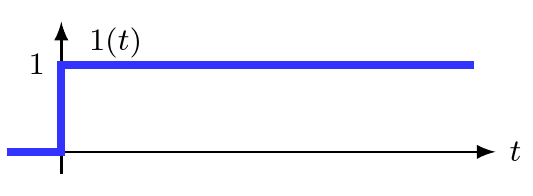
\includegraphics[width=0.25\linewidth, valign=c]{Images/Scalino.png}
        \\
        $\mathcal{L}[t \cdot 1(t)]=\dfrac{1}{s^2}$ & 
        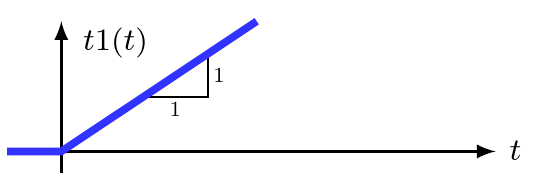
\includegraphics[width=0.25\linewidth, valign=c]{Images/Scalino_2.png}
        \\
        $\mathcal{L}[e^{\alpha t} \cdot 1(t)]=\dfrac{1}{s-\alpha}$ & 
        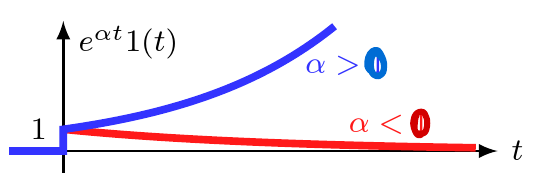
\includegraphics[width=0.25\linewidth, valign=c]{Images/Scalino_3.png}\\
    \end{tabular}
\end{center}

\subsubsection{Trasformata della delta}
\begin{align*}
    \mathcal{L}[\delta(t)] &= \int_{0^-}^{+\infty} \delta(t) e^{-st} \ dt \\
    &= \int_{0^-}^0 \delta(t) \underbrace{e^{-s\cdot 0}}_{1} \ dt + \underbrace{\int_{0^+}^{+\infty} \underbrace{\delta(t)}_{0} e^{-st} \ dt}_{0} \\
\end{align*}

\subsubsection{Trasformata del segnale gradino unitario}
Il segnale gradin unitario $1(t)$ è definito
\begin{equation}
    1(t) = \begin{cases}
        0 &t<0\\
        1 &t\geq 0
    \end{cases}
\end{equation}
\begin{align*}
    \int_{0^-}^{+ \infty} 1(t)e^{-st} \ dt &= \int_{0}^{+ \infty} \underbrace{1(t)}_{1}e^{-st} \ dt\\
    &= \int_{0}^{+ \infty}e^{-st} \ dt\\
    &= \frac{e^{-st}}{-s}\bigg|_{t\rightarrow+\infty} - \frac{e^{-0}}{-s}\bigg|_{t=0}
\end{align*}
$\lim_{t\rightarrow+\infty}e^{-st}=0$, $e^0=1$
\begin{equation}
    \underbrace{\frac{\overbrace{e^{-st}}^{0}}{-s}}_{0}\bigg|_{t\rightarrow+\infty} - \frac{\overbrace{e^{-0}}^{1}}{-s}\bigg|_{t=0} = \frac{1}{s}
\end{equation}

\subsubsection{Trasformata del segnale rampa}
Il segnale \textit{rampa} $r(t)$ è definito come
\begin{equation}
    r(t) = \begin{cases}
        0 &t<0\\
        t &t\geq 0
    \end{cases} \ \ \ \ \  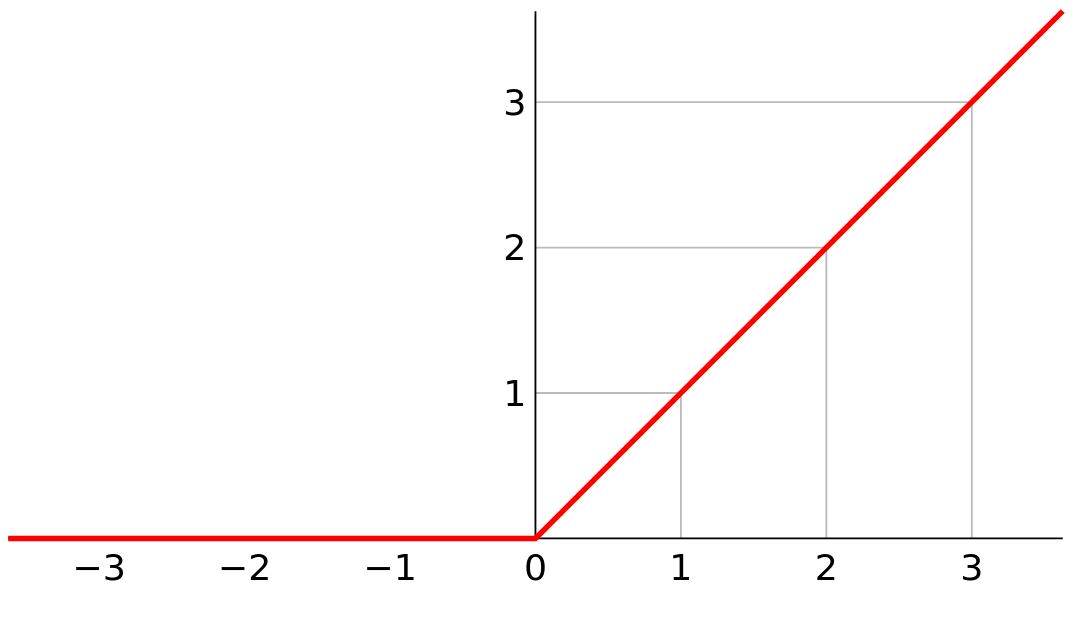
\includegraphics[width=0.25\linewidth, valign=c]{Images/Segnale_rampa.png}
\end{equation}
Per calcolare la trasformata del segnale rampa utilizziamo la proprietà di \nameref{Derivazione nel dominio della variabile complessa}
\begin{align*}
    \mathcal{L}[t \cdot 1(t)] &= -\frac{d\left(\dfrac{1}{s}\right)}{ds}\\
    &= \frac{1}{s^2}
\end{align*}
\vspace*{0.2cm}\\
Mentre per calcolare la trasformata del gradino moltiplicato un esponenziale utilizziamo la proprietà di \nameref{Traslazione nel dominio della variabile complessa}
\begin{align*}
    \mathcal{L}[e^{\alpha t} \underbrace{1(t)}_{f(t)}] &= \underbrace{F(s-\alpha)}_{F(s)=\frac{1}{s}}\\
    &= \frac{1}{s-\alpha}
\end{align*}

\subsection{Tabella trasformate}

\begin{center}
    \renewcommand{\arraystretch}{5}
    \begin{tabular}{c c}
        $\mathcal{L}[\delta(t)]=1$ & 
        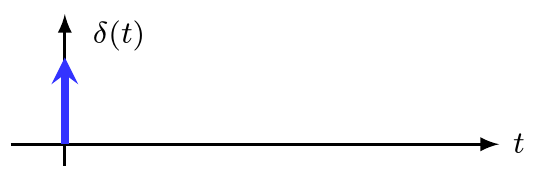
\includegraphics[width=0.25\linewidth, valign=c]{Images/Delta.png}
        \\
        $\mathcal{L}[1(t)]=\dfrac{1}{s}$ & 
        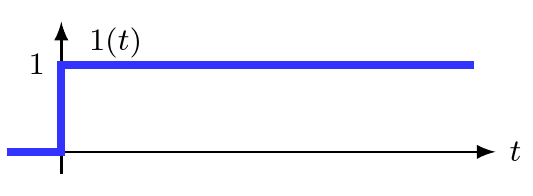
\includegraphics[width=0.25\linewidth, valign=c]{Images/Scalino.png}
        \\
        $\mathcal{L}[t \cdot 1(t)]=\dfrac{1}{s^2}$ & 
        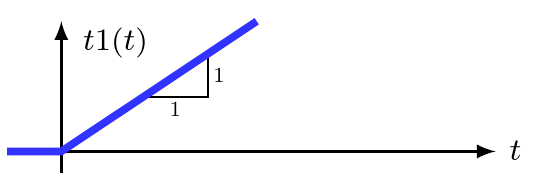
\includegraphics[width=0.25\linewidth, valign=c]{Images/Scalino_2.png}
        \\
        $\mathcal{L}[e^{\alpha t} \cdot 1(t)]=\dfrac{1}{s-\alpha}$ & 
        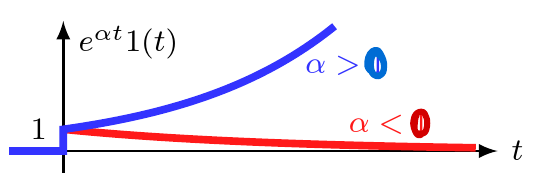
\includegraphics[width=0.25\linewidth, valign=c]{Images/Scalino_3.png}\\
        $\mathcal{L}[\sin(\omega t)1(t)]= \dfrac{\omega}{s^2+\omega^2}$ & 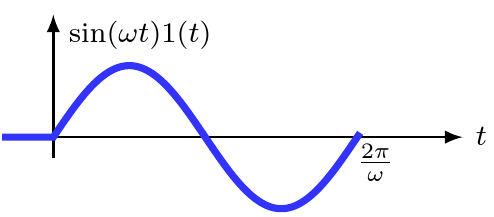
\includegraphics[width=0.25\linewidth, valign=c]{Images/Trasformata_seno.png}\\
        $\mathcal{L}[\cos(\omega t)1(t)]= \dfrac{\omega}{s^2+\omega^2}$ & 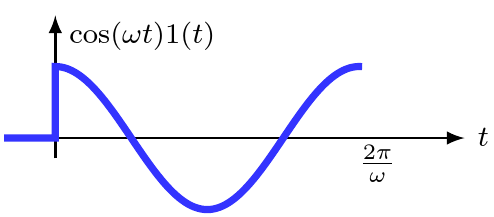
\includegraphics[width=0.25\linewidth, valign=c]{Images/Trasformata_coseno.png}\\
        $\mathcal{L}[\sin(\omega t + \varphi)1(t)]= \dfrac{\omega \cos\varphi \pm s \sin\phi}{s^2+\omega^2}$\\
        $\mathcal{L}[\cos(\omega t + \varphi)1(t)]= \dfrac{s \cos\phi \mp \omega \sin\varphi}{s^2+\omega^2}$
    \end{tabular}
\end{center}



\section{Funzione di trasferimento}
\subsection{Introduzione}
Consideriamo il sistema LTI con $x\in \mathbb{R}^n, u\in \mathbb{R}^m,y\in \mathbb{R}^p$
\begin{align*}
    \dot x(t) &= Ax(t) + Bu(t)\\
    y(t) &= Cx(t) + Du(t)
\end{align*}
con $x(0) = x_0$.
\vspace*{0.1cm}\\
Siano $X(s):= \mathcal{L}[x(t)], U(s):= \mathcal{L}[u(t)]$ e $Y(s):= \mathcal{L}[y(t)]$. Applichiamo la trasformazione di Laplace ad ambo i membri delle equazioni precedenti, ricordando che $\mathcal{L}\left[\dfrac{d}{dt}x(t)\right]=sX(s)-x(0)$
\begin{align*}
    sX(s) - x(0) &= AX(s) + BU(s)\\
    Y(s) &= CX(s) + DU(s) 
\end{align*}
se raccolgo $X(s)$ nella prima equazione
\begin{align*}
    (sI-A)X(s) &=x_0+ BU(s)\\
    Y(s) &= CX(s) + DU(s) 
\end{align*}
\begin{align*}
    X(s) &=\overbrace{(sI-A)^{-1}x_0}^{X_\ell (s)} +\overbrace{(sI-A)^{-1} BU(s)}^{X_f (s)}\\
    Y(s) &= CX(s) + DU(s) 
\end{align*}
Sottolineiamo che se avessimo un sistema generico non si potrebbe riscrivere come abbiamo fatto perché \underline{le matrici devono essere} \underline{costanti}.\\
Inoltre per poter scrivere un sistema LTI come sopra la matrice $(sI-A)$ deve essere invertibile; una matrice è invertibile se il suo determinante è non nullo, quindi, se $s$ è autovalore della matrice della dinamica e $p(s)$ è il polinomio caratteristico associato:
\begin{equation}
    p(s) = \det (sI-A)
\end{equation}
Quindi le trasformate dello stato e dell'uscita del sistema in funzione di $x_0$ e $U(s)$ sono 
\begin{align*}
    X(s) &=\overbrace{(sI-A)^{-1}x_0}^{\T{evoluzione libera}} +\overbrace{(sI-A)^{-1} BU(s)}^{\T{evoluzione forzata}}\\
    Y(s) &=\underbrace{C(sI-A)^{-1}x_0}_{\T{evoluzione libera}} + \underbrace{\left(C(sI-A)^{-1}B+D\right)U(s)}_{\T{evoluzione forzata}}
\end{align*}
\begin{align*}
    X_\ell(s) &= (sI-A)^{-1}x_0 & X_f(s) &= (sI-A)^{-1} BU(s)\\
    Y_\ell(s) &= C(sI-A)^{-1}x_0 & Y_f(s) &= \left(C(sI-A)^{-1}B+D\right)U(s)  
\end{align*}
Consideriamo ora la trasformata dell'evoluzione forzata dell'uscita
\begin{equation*}
    Y_f(s) = \left(C(sI-A)^{-1}B+D\right) U(s)
\end{equation*}
la matrice
\begin{equation*}
    G(s) = C(sI-A)^{-1}B+D
\end{equation*}
è detta \textit{funzione di trasferimento}; se il sistema è SISO (Single Input Single Output) è una funzione scalare.
\vspace*{0.1cm}\\
Abbiamo così ottenuto una \textbf{rappresentazione ingresso-uscita}
\begin{equation}
    Y_f(s) = G(s)U(s)
\end{equation}
se assumiamo che $x(0)=0$ otteniamo esattamente la trasformata di Laplace dell'uscita $y$
\begin{equation}\label{funzione di trasferimento}
    Y(s) = G(s)U(s)
\end{equation}
Due osservazioni:
\begin{itemize}[label=$\triangleright$]
    \item se si conosce la funzione di trasferimento $G(s)$ di un sistema e la trasformata di Laplace $U(s)$ dell'ingresso, è possibile calcolare, mediante antitrasformazione dell'equazione precedente \ref{funzione di trasferimento}, il movimento forzato $y_f$ dell'uscita (che ovviamente coincide con il movimento $y$ se lo stato iniziale è nullo);
    \item la funzione di trasferimento è data dal rapporto tra la trasformata dell'uscita e dell'ingresso nel caso di $x(0)=0$
    \begin{equation}
        G(s) = \frac{Y(s)}{U(s)}
    \end{equation}
\end{itemize}

\subsubsection{Richiami di calcolo matriciale}

\subsubsection{Matrice diagonale}
Una \textit{matrice diagonale} è una matrice quadrata tale che per $i \neq j$ si ha sempre $a_{ij}=0$ (ogni matrice diagonale è simmetrica).
$$ \begin{pmatrix} 1&0&0&0 \\ 0&7&0&0 \\ 0&0&9&0 \\ 0&0&0&-3  \end{pmatrix}, \ \begin{pmatrix} 0&0&0&0 \\ 0&2&0&0 \\ 0&0&3&0 \\ 0&0&0&1  \end{pmatrix} $$


\subsubsection{Matrice triangolare alta}
Una \textit{matrice triangolare alta} è una matrice quadrata tale che per $i>j \ \  a_{ij}=0$
$$ \begin{pmatrix} a_{11}&a_{12}&a_{13}&a_{14} \\ a_{21}&a_{22}&a_{23}&a_{24} \\ a_{31}&a_{32}&a_{33}&a_{34} \\ a_{41}&a_{42}&a_{43}&a_{44} \end{pmatrix} \rightarrow \begin{pmatrix} 1&4&-3&7 \\ 0&6&-8&9\\ 0&0&3&-5 \\ 0&0&0&1 \end{pmatrix}   $$


\subsubsection{Matrice triangolare bassa}
Una \textit{matrice triangolare alta} è una matrice quadrata tale che per $i<j \ \  a_{ij}=0$
$$ \begin{pmatrix} a_{11}&a_{12}&a_{13}&a_{14} \\ a_{21}&a_{22}&a_{23}&a_{24} \\ a_{31}&a_{32}&a_{33}&a_{34} \\ a_{41}&a_{42}&a_{43}&a_{44} \end{pmatrix} \rightarrow \begin{pmatrix}  1&0&0&0 \\ 6&7&0&0 \\ 3&-2&-9&0 \\ 5&4&-8&3 \end{pmatrix}   $$
Nota: una matrice diagonale è triangolare alta e triangolare bassa.


\subsubsection{Matrice identità}
$$ I_n = \begin{pmatrix}
1 & 0 & .. & 0\\
0 & .. & .. & .. \\
.. & .. & .. & ..  \\
0 & .. & .. & 1
\end{pmatrix} I_2 = \begin{pmatrix} 1 & 0 \\ 0 & 1 \end{pmatrix} $$


\subsubsection{Trasposta di una matrice}
$$\begin{pmatrix}
2 & 1 & 7 \\
4 & 0 & 2
\end{pmatrix}^T = \begin{pmatrix}2 & 4 \\ 1 & 0 \\ 7 & 2 \end{pmatrix} $$
$A = (a_{ij})$ significa che l'elemento di posto $(i,j)$ in $A$ è $a_{i,j}$.
\vspace{0.2cm}\\
$A^T := B = (b_{ij})$ con $b_{ij} = a_{ji}$ per ogni coppia di indici $(i,j)$.
















































\end{document}
